% ******************************* PhD Thesis Template **************************
% Please have a look at the README.md file for info on how to use the template

\documentclass[a4paper,12pt,times,numbered,print,index]{PhDThesisPSnPDF}

% ******************************************************************************
% ******************************* Class Options ********************************
% *********************** See README for more details **************************
% ******************************************************************************

% `a4paper'(The University of Cambridge PhD thesis guidelines recommends a page
% size a4 - default option) or `a5paper': A5 Paper size is also allowed as per
% the Cambridge University Engineering Deparment guidelines for PhD thesis
%
% `11pt' or `12pt'(default): Font Size 10pt is NOT recommended by the University
% guidelines
%
% `oneside' or `twoside'(default): Printing double side (twoside) or single
% side.
%
% `print': Use `print' for print version with appropriate margins and page
% layout. Leaving the options field blank will activate Online version.
%
% `index': For index at the end of the thesis
%
% `draftclassic': For draft mode without loading any images (same as draft in book)
%
% `draft': Special draft mode with line numbers, images, and water mark with
% timestamp and custom text. Position of the text can also be modified.
%
% `abstract': To generate only the title page and abstract page with
% dissertation title and name, to submit to the Student Registry
%
% `chapter`: This option enables only the specified chapter and it's references
%  Useful for review and corrections.
%
% ************************* Custom Page Margins ********************************
%
% `custommargin`: Use `custommargin' in options to activate custom page margins,
% which can be defined in the preamble.tex. Custom margin will override
% print/online margin setup.
%
% *********************** Choosing the Fonts in Class Options ******************
%
% `times' : Times font with math support. (The Cambridge University guidelines
% recommend using times)
%
% `fourier': Utopia Font with Fourier Math font (Font has to be installed)
%            It's a free font.
%
% `customfont': Use `customfont' option in the document class and load the
% package in the preamble.tex
%
% default or leave empty: `Latin Modern' font will be loaded.
%
% ********************** Choosing the Bibliography style ***********************
%
% `authoryear': For author-year citation eg., Krishna (2013)
%
% `numbered': (Default Option) For numbered and sorted citation e.g., [1,5,2]
%
% `custombib': Define your own bibliography style in the `preamble.tex' file.
%              `\RequirePackage[square, sort, numbers, authoryear]{natbib}'.
%              This can be also used to load biblatex instead of natbib
%              (See Preamble)
%
% **************************** Choosing the Page Style *************************
%
% `default (leave empty)': For Page Numbers in Header (Left Even, Right Odd) and
% Chapter Name in Header (Right Even) and Section Name (Left Odd). Blank Footer.
%
% `PageStyleI': Chapter Name next & Page Number on Even Side (Left Even).
% Section Name & Page Number in Header on Odd Side (Right Odd). Footer is empty.
%
% `PageStyleII': Chapter Name on Even Side (Left Even) in Header. Section Number
% and Section Name in Header on Odd Side (Right Odd). Page numbering in footer

% Uncomment to change page style
%\pagestyle{PageStyleII}

% ********************************** Preamble **********************************
% Preamble: Contains packages and user-defined commands and settings
% ******************************************************************************
% ****************************** Custom Margin *********************************

% Add `custommargin' in the document class options to use this section
% Set {innerside margin / outerside margin / topmargin / bottom margin}  and
% other page dimensions
\ifsetCustomMargin
  \RequirePackage[left=37mm,right=30mm,top=35mm,bottom=30mm]{geometry}
  \setFancyHdr % To apply fancy header after geometry package is loaded
\fi

% Add spaces between paragraphs
%\setlength{\parskip}{0.5em}
% Ragged bottom avoids extra whitespaces between paragraphs
\raggedbottom
% To remove the excess top spacing for enumeration, list and description
%\usepackage{enumitem}
%\setlist[enumerate,itemize,description]{topsep=0em}

% *****************************************************************************
% ******************* Fonts (like different typewriter fonts etc.)*************

% Add `customfont' in the document class option to use this section

\ifsetCustomFont
  % Set your custom font here and use `customfont' in options. Leave empty to
  % load computer modern font (default LaTeX font).
  %\RequirePackage{helvet}

  % For use with XeLaTeX
  %  \setmainfont[
  %    Path              = ./libertine/opentype/,
  %    Extension         = .otf,
  %    UprightFont = LinLibertine_R,
  %    BoldFont = LinLibertine_RZ, % Linux Libertine O Regular Semibold
  %    ItalicFont = LinLibertine_RI,
  %    BoldItalicFont = LinLibertine_RZI, % Linux Libertine O Regular Semibold Italic
  %  ]
  %  {libertine}
  %  % load font from system font
  %  \newfontfamily\libertinesystemfont{Linux Libertine O}
\fi

% *****************************************************************************
% **************************** Custom Packages ********************************

% ************************* Algorithms and Pseudocode **************************

%\usepackage{algpseudocode}


% ********************Captions and Hyperreferencing / URL **********************

% Captions: This makes captions of figures use a boldfaced small font.
%\RequirePackage[small,bf]{caption}

\RequirePackage[labelsep=space,tableposition=top]{caption}
\renewcommand{\figurename}{Fig.} %to support older versions of captions.sty


% *************************** Graphics and figures *****************************

%\usepackage{rotating}
%\usepackage{wrapfig}

% Uncomment the following two lines to force Latex to place the figure.
% Use [H] when including graphics. Note 'H' instead of 'h'
%\usepackage{float}
%\restylefloat{figure}

% Subcaption package is also available in the sty folder you can use that by
% uncommenting the following line
% This is for people stuck with older versions of texlive
%\usepackage{sty/caption/subcaption}
%\usepackage{subcaption}

% ********************************** Tables ************************************
\usepackage{booktabs} % For professional looking tables
\usepackage{multirow}

%\usepackage{multicol}
%\usepackage{longtable}
%\usepackage{tabularx}


% *********************************** SI Units *********************************
\usepackage{siunitx} % use this package module for SI units

%diennv

%\usepackage[export]{adjustbox}
%\usepackage{url}
%\usepackage{amsmath,amssymb,amsfonts}
%\usepackage{algorithmic}
%\usepackage{graphicx}
%\usepackage{textcomp}
%\usepackage{float}
\usepackage{subfig}
%\usepackage{gensymb}
%\usepackage[]{multirow}
%\usepackage[]{siunitx}
%\usepackage[]{booktabs}
%\usepackage{array, multirow, tabularx, booktabs}
\usepackage{algorithmic}
\usepackage[]{algorithm2e}
\SetKwInput{kwInit}{Init}
\usepackage{array}
%\usepackage{siunitx}
%\usepackage{subcaption}


% ******************************* Line Spacing *********************************

% Choose linespacing as appropriate. Default is one-half line spacing as per the
% University guidelines
%diennv
 \doublespacing
% \onehalfspacing
% \singlespacing


% ************************ Formatting / Footnote *******************************

% Don't break enumeration (etc.) across pages in an ugly manner (default 10000)
%\clubpenalty=500
%\widowpenalty=500

%\usepackage[perpage]{footmisc} %Range of footnote options


% *****************************************************************************
% *************************** Bibliography  and References ********************

%\usepackage{cleveref} %Referencing without need to explicitly state fig /table

% Add `custombib' in the document class option to use this section
\ifuseCustomBib
   \RequirePackage[square, sort, numbers, authoryear]{natbib} % CustomBib

% If you would like to use biblatex for your reference management, as opposed to the default `natbibpackage` pass the option `custombib` in the document class. Comment out the previous line to make sure you don't load the natbib package. Uncomment the following lines and specify the location of references.bib file

%\RequirePackage[backend=biber, style=numeric-comp, citestyle=numeric, sorting=nty, natbib=true]{biblatex}
%\addbibresource{References/references} %Location of references.bib only for biblatex, Do not omit the .bib extension from the filename.

\fi

% changes the default name `Bibliography` -> `References'
\renewcommand{\bibname}{References}


% ******************************************************************************
% ************************* User Defined Commands ******************************
% ******************************************************************************

% *********** To change the name of Table of Contents / LOF and LOT ************

%\renewcommand{\contentsname}{My Table of Contents}
%\renewcommand{\listfigurename}{My List of Figures}
%\renewcommand{\listtablename}{My List of Tables}


% ********************** TOC depth and numbering depth *************************

\setcounter{secnumdepth}{2}
\setcounter{tocdepth}{2}


% ******************************* Nomenclature *********************************

% To change the name of the Nomenclature section, uncomment the following line

%\renewcommand{\nomname}{Symbols}


% ********************************* Appendix ***********************************

% The default value of both \appendixtocname and \appendixpagename is `Appendices'. These names can all be changed via:

%\renewcommand{\appendixtocname}{List of appendices}
%\renewcommand{\appendixname}{Appndx}

% *********************** Configure Draft Mode **********************************

% Uncomment to disable figures in `draft'
%\setkeys{Gin}{draft=true}  % set draft to false to enable figures in `draft'

% These options are active only during the draft mode
% Default text is "Draft"
%\SetDraftText{DRAFT}

% Default Watermark location is top. Location (top/bottom)
%\SetDraftWMPosition{bottom}

% Draft Version - default is v1.0
%\SetDraftVersion{v1.1}

% Draft Text grayscale value (should be between 0-black and 1-white)
% Default value is 0.75
%\SetDraftGrayScale{0.8}


% ******************************** Todo Notes **********************************
%% Uncomment the following lines to have todonotes.

%\ifsetDraft
%	\usepackage[colorinlistoftodos]{todonotes}
%	\newcommand{\mynote}[1]{\todo[author=kks32,size=\small,inline,color=green!40]{#1}}
%\else
%	\newcommand{\mynote}[1]{}
%	\newcommand{\listoftodos}{}
%\fi

% Example todo: \mynote{Hey! I have a note}

% ******************************** Highlighting Changes **********************************
%% Uncomment the following lines to be able to highlight text/modifications.
%\ifsetDraft
%  \usepackage{color, soul}
%  \newcommand{\hlc}[2][yellow]{{\sethlcolor{#1} \hl{#2}}}
%  \newcommand{\hlfix}[2]{\texthl{#1}\todo{#2}}
%\else
%  \newcommand{\hlc}[2]{}
%  \newcommand{\hlfix}[2]{}
%\fi

% Example highlight 1: \hlc{Text to be highlighted}
% Example highlight 2: \hlc[green]{Text to be highlighted in green colour}
% Example highlight 3: \hlfix{Original Text}{Fixed Text}

% *****************************************************************************
% ******************* Better enumeration my MB*************
\usepackage{enumitem}


% ************************ Thesis Information & Meta-data **********************
% Thesis title and author information, refernce file for biblatex
% ************************ Thesis Information & Meta-data **********************
%% The title of the thesis
\title{Towards Scalable Video Analytics using
Compressed-domain Features at the Edge}
%\texorpdfstring is used for PDF metadata. Usage:
%\texorpdfstring{LaTeX_Version}{PDF Version (non-latex)} eg.,
%\texorpdfstring{$sigma$}{sigma}

%% Subtitle (Optional)
%\subtitle{Using the CUED template}

%% The full name of the author
\author{Nguyen Van Dien}

%% Department (eg. Department of Engineering, Maths, Physics)
\dept{Department of Computer Science}

%% University and Crest
\university{Gachon University}
% Crest minimum should be 30mm.
\crest{
\includegraphics[width=0.2\textwidth]{University_Crest}}
%% Use this crest, if you are using the college crest
%% Crest long miminum should be 65mm
%\crest{
\includegraphics[width=0.45\textwidth]{University_Crest_Long}}

%% College shield [optional] 
% Crest minimum should be 30mm.
%\collegeshield{
\includegraphics[width=0.2\textwidth]{CollegeShields/Kings}}


%% Supervisor (optional)
%% for multiple supervisors, append each supervisor with the \newline command
\supervisor{Prof. Jaehyuk Choi\newline
 Prof. Eun-Seok Ryu}

%% Supervisor Role (optional) - Supervisor (default) or advisor
% \supervisorrole{\textbf{Supervisors: }}
%% if no title is desired:
% \supervisorrole{}

%% Supervisor line width: required to align supervisors
%\supervisorlinewidth{0.35\textwidth}

%% Advisor (optional)
%% for multiple advisors, append each advisor with the \newline command
%\advisor{Dr. A. Advisor\newline
%Dr. B. Advisor}
     
%% Advisor Role (optional) - Advisor (default) or leave empty
% \advisorrole{Advisors: }
%% if no title is required
% \advisorrole{}

%% Advisor line width: required to align supervisors
%\advisorlinewidth{0.25\textwidth}


%% You can redefine the submission text:
% Default as per the University guidelines:
% ``This dissertation is submitted for the degree of''
\renewcommand{\submissiontext}{A dissertation submitted to the department of Computer Science and the committee on graduate studies
of Gachon University in partial fulfillment of the requirements for the degree of Doctor of Philosophy}

%% Full title of the Degree
%\degreetitle{Doctor of Philosophy}

%% College affiliation (optional)
%\college{King's College}

%% Submission date
% Default is set as {\monthname[\the\month]\space\the\year}
%\degreedate{September 2014} 

%% Meta information
\subject{LaTeX} \keywords{{LaTeX} {PhD Thesis} {Engineering} {University of
Cambridge}}


% ***************************** Abstract Separate ******************************
% To printout only the titlepage and the abstract with the PhD title and the
% author name for submission to the Student Registry, use the `abstract' option in
% the document class.

\ifdefineAbstract
 \pagestyle{empty}
 \includeonly{Declaration/declaration, Abstract/abstract}
\fi

% ***************************** Chapter Mode ***********************************
% The chapter mode allows user to only print particular chapters with references
% Title, Contents, Frontmatter are disabled by default
% Useful option to review a particular chapter or to send it to supervisior.
% To use choose `chapter' option in the document class

\ifdefineChapter
 \includeonly{Chapter3/chapter3}
\fi

% ******************************** Front Matter ********************************
\begin{document}

\frontmatter

\maketitle

%% ******************************* Thesis Dedidcation ********************************

\begin{dedication} 

%I would like to dedicate this thesis to my loving parents \dots

\end{dedication}


%% ******************************* Thesis Declaration ***************************

\begin{declaration}

I hereby declare that except where specific reference is made to the work of 
others, the contents of this dissertation are original and have not been 
submitted in whole or in part for consideration for any other degree or 
qualification in this, or any other university. This dissertation is my own 
work and contains nothing which is the outcome of work done in collaboration 
with others, except as specified in the text and Acknowledgements. This 
dissertation contains fewer than 65,000 words including appendices, 
bibliography, footnotes, tables and equations and has fewer than 150 figures.

% Author and date will be inserted automatically from thesis.tex \author \degreedate

\end{declaration}


% ************************** Thesis Acknowledgements **************************

\begin{acknowledgements}       
First, I would like to express my gratitude and appreciation to my major advisor, Dr. Jaehyuk Choi’s mentorship and support, I was able to get access to numerous opportunities, develop myself to be a better researcher, and I hope our cooperation will continue in the future. Thanks to Dr. Eun-Seok Ryu for letting me join the Graduate School to study and research at Gachon University. I also want to thank my committee members: Drs. ???, ???, ???
and Dr. ??? for supporting me complete the PhD program as well as all the valuable inputs to my dissertation. Additionally, the discussions with them helped me broaden my perspective on my research.\\
I am grateful to the support from my parents in VietNam. I thank all my friends at Gachon
for making my life here a happy and precious experience: Le Thanh Tuan, Nguyen Ngoc Quang ... and many others.
Finally, a very special thanks to my wife Tran Thi Thu, a woman who is excellent in
all aspects, beautiful, smart, and generous. I am very grateful for her encouragement,
her patience, and all her love and tenderness.
\end{acknowledgements}

% ************************** Thesis Abstract *****************************
% Use `abstract' as an option in the document class to print only the titlepage and the abstract.
%Every academic paper begins with title page. Its structure depends on the chosen formatting style. An abstract follows it. This is an important part that describes thesis utility. It must be short and take 1-2 paragraphs, about 400 words and contain short summary of results, methods, etc. Here are questions to answer in this part:

%What was the reason to write this paper?
%What thesis statement to prove or disprove?
%What were your instruments? (describe main methods of research)
%What did you find out?
%Why are the results important?
\begin{abstract}
Intelligent Video Analytics(VA) systems have come to play an essential role in many fields, including public safety, transportation safety, and many other industry areas, as automated tools for data extracting and analyzing huge datasets such as multiple live video streams transmitted from a large number of cameras. A key characteristic of such systems is that it is critical to perform real-time analytics so as to provide timely actionable alerts on various tasks, activities and conditions. Due to the computation-intensive and bandwidth-intensive nature of these operations, however, video analytics servers may not fulfill the requirements when serving for a large number of cameras simultaneously. To handle these challenges, this dissertation present an edge-computing based system that minimizes transfer of video data from the surveillance camera feeds on a cloud video analytics server. Based on a novel approach of utilizing the information from the encoded bitstream, the edge can achieve low processing complexity of object tracking in surveillance videos and filters non-motion frames from the list of data which will be forwarded to the cloud server. To demonstrate the effectiveness of the approach, we have implemented a video surveillance prototype consisting of edge devices with low computational capacity and a GPU-enabled server. The evaluation results show that our method can efficiently catch the characteristics of the frame and is compatible with the edge-to-cloud platform in terms of accuracy and delay sensitivity. The average processing time of this method is approximately 39 ms/frame with high definition resolution video, which outperforms most of the state of art method. In addition to scenario implementation of the proposed system, the method helps the cloud server reduce 49\% load of GPU, 49\% load of CPU, and 55\% of network traffic while maintaining the accuracy of real-time video analytics event detection.
\end{abstract}


% *********************** Adding TOC and List of Figures ***********************

\tableofcontents

\listoffigures

\listoftables

% \printnomenclature[space] space can be set as 2em between symbol and description
%\printnomenclature[3em]

\printnomenclature

% ******************************** Main Matter *********************************
\mainmatter

%!TEX root = ../thesis.tex
%*******************************************************************************
%*********************************** First Chapter *****************************
%*******************************************************************************
%The first big part is the introduction. It may seem similar to an abstract. It pursues different goals –reader hooking, providing background information and logical transition to your own research. Here is what you need to disclose in this chapter:

%Enough background information about previous researches should be presented to make readers understand place of text in science system.
%Give an explanation concerning contents – what will be included into thesis.
%Provide readers with verbal ‘road maps’.
%Cite previous works. The citations must be related to text’s goals. Do not list everything you have read about subject.
%These sections must take three pages of paper, excluding contents and table lists.

\chapter{Introduction}  %Title of the First Chapter
%********************************** %First Section  **************************************
\begin{figure*}
\centering
\subfloat[]
{
    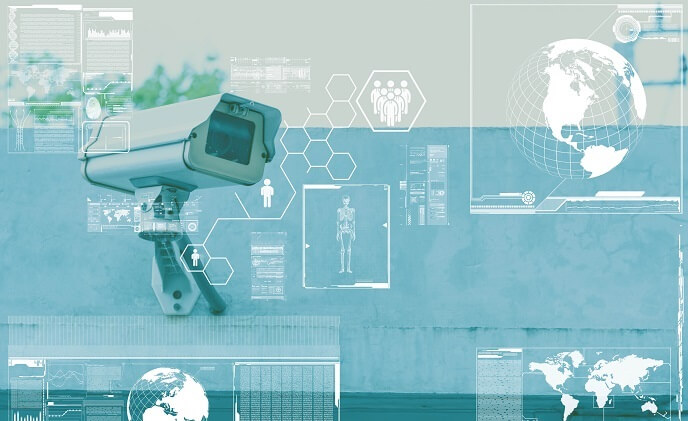
\includegraphics[scale=0.3]{Figures/cctv1.jpg}
}
\subfloat[]
{
    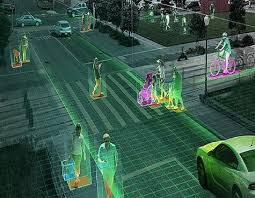
\includegraphics[scale=0.64]{Figures/cctv2.jpg}
}
\caption{Surveillance Camera Deployment and Application}
\label{fig:cctv}
\end{figure*}
Today the world is witnessing an exponential increase in camera deployment ~\citep{ananthanarayanan2019demo} as shown in Figure \ref{fig:cctv} with cities and organizations steadily increasing the size and reach of their deployments. For example, cities now deploy tens thousands of cameras, each continually collecting and streaming rich video data \cite{ref0}, \cite{ref1}, \cite{ref2}. According to IHS Markit’s annual report \cite{oliverreport}, as of 2018, China has one camera for each 4.1 people in the country and the United State has a people-to-camera ratio of 4.6-to-1. The massive deployments of cameras are brought on mainly by the growth of the video surveillance industry due to increasing concerns about public safety and security. With such prevalent trend, intelligent video analytics systems have been playing an essential role, performing important task in various fields including surveillance, transportation, manufacturing, etc.
Video analytics software analyzes videos in order to detect events the system is programmed to look for – when something is moving in front of the camera.These systems analyze video feeds to guide long-running tasks such as traffic monitoring, customer tracking, and surveillance. Key to the success of such applications has been recent advances in computer vision, particularly neural network based techniques for highly accurate object detection and recognition \cite{cai2015learning}, \cite{krizhevsky2017imagenet}, \cite{li2015convolutional}.\\
In a typical real-time video analytics pipeline as 
\begin{figure*}
\centering
 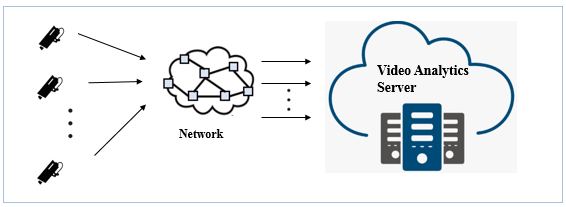
\includegraphics[width=1.0\linewidth]{Figures/cloud.png}
 \caption{Overall of cloud based video analytics server}
 \label{fig:overall}
\end{figure*}
Figure \ref{fig:overall} illustrates a traditional cloud-based video stream analytics system. A large number of camera transfer video data to a central cloud (datacenter) where video analytics is performed. However, this traditional approach makes it difficult to perform real-time analytics on live video streams from many cameras because the video analytics involves several computation-intensive tasks such as object detection, object tracking, object recognition and so on. Besides, streaming video from multiple camera to the cloud consumes a lot of network bandwidth over limited-bandwidth networks, which leads to high latency, causing significant challenge for real-time video analytics.\\
Significant work has been expended to improve the efficiency of video analytics pipelines \cite{canel2019scaling}, \cite{chen2015glimpse}, \cite{hsieh2018focus}, \cite{jiang2018chameleon}. Accross these systems, a prevailing (and natural) strategy is to improve efficiency by filtering out frames that do not contain relevant information for the query using the additional edge devices. In this study, to address the question of how to overcome this network bottleneck and offload large volumes of data from a distributed camera deployment in real-time to a datacenter for further processing, we aim to develop a solution by harnessing edge computing.
Video analytics at the edge has multiple benefits such as decreasing the response time, saving network bandwidth, and minimizing the peak workload to the cloud. 
\begin{figure*}
\centering
 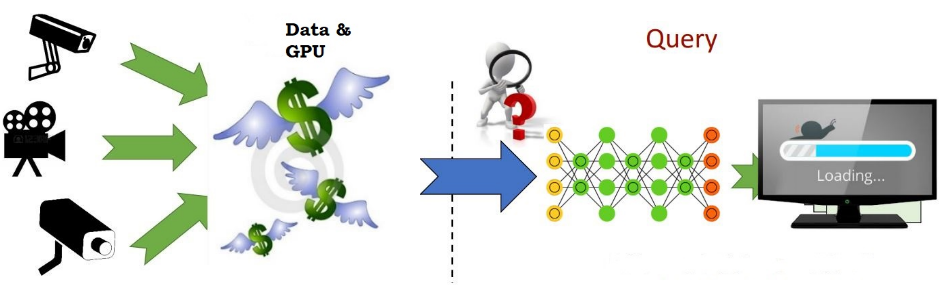
\includegraphics[width=1.0\linewidth]{Figures/vachallenge.png}
 \caption{Real-time Video Analytics Challenges}
 \label{fig:chal}
\end{figure*}
In previous works, the solutions are based on either:
\begin{itemize}
\item Binary classification model: eliminate frames that do not contain an object of interest.
\item Simple frame differencing: eliminate frames whose low-level
features (e.g., pixel values) have not changed substantially.
\end{itemize}
Typically, exist systems use deep-learning framework to understand video frame context. Video frame is analyzed on pixel domain which require fully video decoding. However, edge devices are typically much less powerful than the cloud, with limited computing resources such as a few GPUs (graphics processing units) and CPUs (central processing units), as well as smaller RAM (Random Access Memory) capacities \cite{stone2019towards}. In the field of public safety, the ability to simultaneously process multiple feeds and provide real-time video analytics is critical. Thus, this study seeks to answers how edge devices and the cloud can cooperate in an efficient manner to achieve real-time and scalable video analytics. Our motivation is based on the observation that surveillance camera images are unchanged for a long time and video content is often quite redundant. So, it is undesirable to conduct analytics on redundant video frames from cameras, leading to increase latency and system expense by a waste of network bandwidth, computing resources and power consumption in the cloud as described in Figure \ref{fig:chal}. \\
\begin{figure*}
\centering
 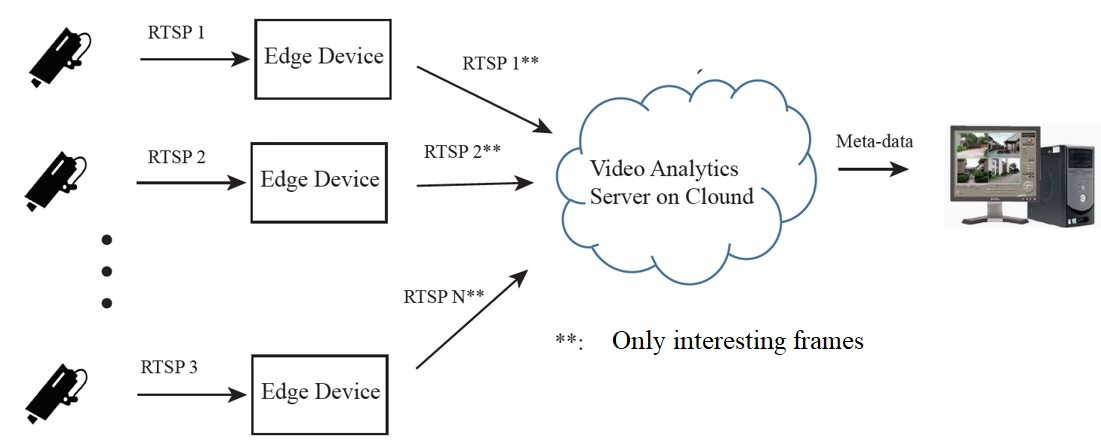
\includegraphics[width=1.0\linewidth]{Figures/motivation.jpg}
 \caption{The motivated system design}
 \label{fig:mot}
\end{figure*}
 Motivated by this, we propose a pre-process module that acts as a video filter function at the edge device to eliminate the redundant static images before feeding videos to the cloud for further analysis as described in Figure \ref{fig:mot}. The proposed method is driven by the compressed-domain feature which doest not require GPU-based processing and fully video decoing. Therefore, it is light-weight method and cheap solution. The  method runs on an edge device and recognizes the motions (i.e., moving objects) in the consecutive video frames. Based on the motion recognition result, our module decides whether to pass the video frame to the cloud or filter it out. As a result, the proposed motion-based filtering module can reduce not only computational load of the cloud nodes but also network traffic to the cloud. \\
Motion recognition schemes can be classified into two categories: (i) video pixel-domain based and (ii) video compressed-domain based approaches. In pixel-domain based approaches \cite{lu2014moving}, \cite{kumar2016segmentation}, \cite{gujrathi2014detecting}, \cite{wang2019ground} video is completely decoded before using background modelling or vision based deep learning framework to detect moving objects at the pixel level. The performance of video pixel-domain processing in large systems may be challenged by the load of decoding multiple streams and the image pixel-based calculation. Thus, pixel-based approach requires higher computational complexity and can make it difficult to fulfill the real-time requirement of edge devices. 
Compressed-domain approaches \cite{favalli2000object},\cite{yoneyama1999moving},\cite{dong2006object},\cite{achanta2002compressed} rely on video coding artifacts of compressed bitstreams such as motion vector (MV), macroblock partitions, and quantization coefficients for recognizing motion. Compared to pixel-domain based algorithms, compressed-domain methods generally require less computational resources because analyzing input information is already possible in the bitstream.\\ In this study, we proposed a compressed-domain based moving objects detection that applies a data clustering and an intersection of union (IoU) rate-based object tracking technique of computer vision. Using only MVs, which are provided by video encoders in a compressed bitstream, our approach is able to efficiently detect moving objects. Furthermore, an experimental evaluation of our method is provided to compare it with the state-of-the-art compressed-domain tracking methods in term of processing time, and demonstrate its functionalities to evaluate the efficiency of the proposed edge device with a cloud video analytics server in a real-world scenario. In summary, this study makes the following contributions.
\begin{itemize}
\item Utilizing Video Coding Motion Vectors (MV) analysis to filter out the static frames from video stream.
\item Introduction of a compressed-domain moving objects detection method that can be applied for numerous surveillance applications.
\item Design an edge-to-cloud computing system for surveillance video analytics that applies the proposed method at edge devices to minimize the transfer of video data from surveillance camera feeds to the cloud.
\item Implementation and evaluation of the proposed method on cheap edge device (Pi4 ) and achieve real-time processing time of  39 ms/frame with high definition resolution video.
\end{itemize}
%
\nomenclature[z-VMS]{VMS}{Video Management Software}
\nomenclature[z-VA]{VA}{Video Analytics}
\nomenclature[z-CCTV]{CCTV}{Closed Circuit Television}
\nomenclature[z-CNN]{CNN}{Convolutional Neural Networks}
\nomenclature[z-FPS]{FPS}{Frames Per Second}
\nomenclature[z-MV]{MV}{Motion Vector}
\nomenclature[z-AVC]{AVC}{Advanced Video Coding}
\nomenclature[z-RTSP]{RTSP}{Real-Time Streaming Protocol}
\nomenclature[z-MCP]{MCP}{Motion-Compensated Prediction}
\nomenclature[z-HEVC]{HEVC}{High Efficiency Video Coding}
\nomenclature[z-R-CNN]{R-CNN}{Regions with CNN}
\nomenclature[z-SSD]{SSD}{Single Shot Multi-box Detector}
\nomenclature[z-YOLO]{YOLO}{You Only Look Once}
\nomenclature[z-CPU]{CPU}{Central Processing Unit}
\nomenclature[z-GPU]{GPU}{Graphics Processing Unit}
\nomenclature[z-RAM]{RAM}{Random Access Memory}
\nomenclature[z-CUDA]{CUDA}{Compute Unified Device Architecture}
\nomenclature[z-IOU]{IoU}{Intersection Over Union}
%
\chapter{Background}
%Before explaining the proposed VA design, the background information necessary to understanding VA architecture is described %briefly, followed by a short summary of state-of-art algorithms for object detection used in our proposed VA.
Object detection in images and videos has received a lot of attention of video analytics researchers in recent years. There are many different approaches to detect video moving object, both utilizing compressed and uncompressed video domain. In this chapter, we briefly introduce the current state-of-the-art approaches for moving object detection on both compressed domain and pixel domain. In addition, the background information necessary to understanding VA architecture is described briefly.
\section{Surveillance Video Analytics Architectures and Challenges}
\begin{figure*}
\centering
\subfloat[]
{
    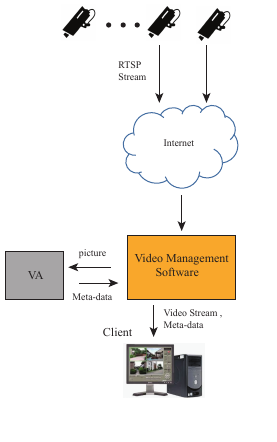
\includegraphics[scale=0.6]{Figures/Va-neta.png}
    \label{fig:va_a}
}
\subfloat[]
{
    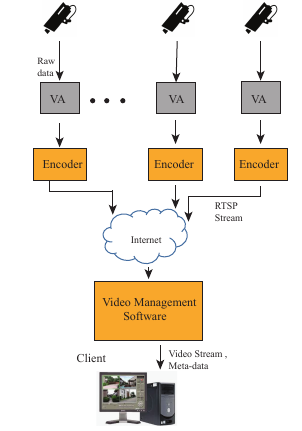
\includegraphics[scale=0.6]{Figures/Va-netb.png}
    \label{fig:va_b}
}
\caption{Video Analytics Implementation, (a) Video management server based implementation, (b) Edge camera based implementation}
\label{fig:va_arch}
\end{figure*}
Video surveillance systems are normally built using the following main components: surveillance IP cameras, VMS, device storage and VA modules (optional). VA can be implemented in two main configurations, as discussed below.
\subsection{Edge Camera Based Deployment}
In this approach, the VA is deployed through a  camera device or video encoder \cite{chen2017smart} such as that shown in Figure \ref{fig:va_b}, which must have enough the processing power to run the VA functionality. Hence it is an expensive and challenging approach to wide-area video processing. This approach seems ideal, however it does not perform satisfactorily in many cases because of the limitations on the overall surveillance system design and performance. Most surveillance camera device still lack sufficient processing power for highend VA requirements, and therefore, this approach has many drawbacks in real-world deployment. 
\subsection{Video Management Server Based Implementation}
In this approach, as shown in Figure \ref{fig:va_a}, VA is implemented through a dedicated server that pulls the video from the camera devices or from VMS, analyzes it, and issues analysis results. However, it has some challenges, which are listed below:
\begin{itemize}
\item “The VA server requires the video to be transmitted and therefore causes an increase in network traffic congestion. In detail, running video analytics by forwarding all video to the cloud overloads with the bandwidth constraints of some deployments, which do uploading all camera data. Each camera’s uplink bandwidth is limited, both by the physical constraints of network components such as: cable, switch, router.. Specifically, we consider large-scale deployments where each camera receives a bandwidth allocation of a few hundred kilobits per second, or less. For comparison, a low-quality H.264-encoded 1080p (1920×1080 pixels) stream is approximately 2 Mbits/s, an order of magnitude greater than our available uplink bandwidth. Yet, such low-quality data is often insufficient to perform accurate analysis: Modern 4K (3840×2160 pixels) cameras produce up to 30 to 40 Mbits/s. An edge-based filter answers this challenge with semantic filtering that uploads only frames that are relevant to applications”.
\item “The video data quality analyzed by the VA server is usually degraded because of lossly compression and transmission effects, and therefore”.
\item “The VA server is limited by its processing power, which makes it infeasible for large scale surveillance installations which deploy hundreds (and increasingly thousands) of cameras requiring a variety of VA functionalities. For example, a Full HD (1080P) stream at 30 FPS is $\approx$ 1.4 Gb/s when decompressed. Accomplishing VA at scale requires abundant compute, memory resources, so existing systems often perform this processing in the cloud, using GPUs”.
\end{itemize}
However, this approach is independent with surveillance camera sources, and is therefore applicable to most types of surveillance systems, and recent technological developments can reduce the effect of the above drawbacks. For example, the release of high definition video surveillance footage with resolutions up to 1080p will decrease the impact of the image quality degradation during codec processing and by releasing the new video coding standard as well as the transcoder \cite{thanh2019efficient}, high efficiency video coding (HEVC)\cite{sullivan2012overview} which has achieved approximately twice the standard compression\cite{ohm2012comparison} will decrease traffic in the network and at the central server, where powerful devices will have sufficient processing power to handle hundreds of camera. Moreover, some edge-based filtering approaches that
is designed to overcome these above issues \cite{canel2019scaling}\cite{li2020reducto}\cite{chen2015glimpse}. These approaches use edge-compute resources allocate with the cameras to identify the video sequences that are necessary to cloud applications and forward only that data for further analysis. By this way, it helps to reduce the wide-area network links bandwidth. In this study, we present an edge-based filter, a system that offers the benefits of ultilizing the both edge  and clound computing to video analytics processing.
\subsection{Video Codec and Video Coding Motion Vectors}
\subsubsection{Video Codec}
\begin{figure*}
\centering
 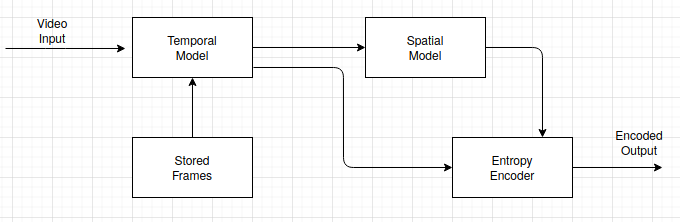
\includegraphics[width=0.8\linewidth]{Figures/encoder.png}
 \caption{Video encoder block diagram.}
 \label{fig:encoder}
\end{figure*}
The previous video coding standards, such as MPEG-1, MPEG-2, H.264 and H.265, are based on block-based motion compensation, transform, quantisation and entropy coding. A video encoder as shown in Figure \ref{fig:encoder} consists of three main functional units: a temporal, a spatial and an entropy encoder. “The input to the temporal model is an uncompressed video sequence. The temporal model tries to reduce temporal redundancy by finding the similarities between neighbouring video frames, normally by constructing a prediction of the current video frame. In MPEG-4 and H.264 codec, the prediction is formed from one or more previous and future frames and is improved by compensating for differences between the frames (motion compressed prediction). The output of the temporal model is a residual frames (created by subtracting operation the prediction from the actual current frame) and a set of model parameters, typicially a set of MVs describing how the motion was compressed. \\
The residual frame formes the input to the spatial model which makes use of similarities between neighbouring samples in the residual frame to reduce spatial redundancy. In MPEG-4 Visual and H.264 this is archieved by applying a transform to the residual samples and quantizing the results. The transform converts the samples into another domain in which they are represented by transform coefficients. The coefficiencents are quantised to remove insignificant values, leaving a small number of significant coefficients that provide a more compact representation of the residual frame. The output of the spatial model is a set of quantised transform coefficients.\\
The entropy encoder compressed the parameters of the temporal model (typically MVs) and the spatial model (coefficients). A compressed sequency consists of coded motion vector parameters, coded residual coefficients and header information.\\
At the decoder, a video frame is reconstructed from the compressed bitstream. The entropy decoder decoded the coefficients and motion vectors are decoded by an entropy decoder to reconstruct a version of the residual frame. The decoder uses the motion vector parameters, together with one or more previously decoded frames, to create a prediction of the current frame and the frame itself is reconstructed by adding the residual frame to this prediction”.
\subsubsection{Video Coding Motion Vectors and Blocked-based Motion Estimation}
	Changes between video frames may caused by object motion (i.e, a human running), camera motion (zoom, rotation) and lighting condition changes.  These changes coresspond to pixel movements between frames. It is able to estimate the trajectory of each pixel through video frames, generating a field of pixel trajectories known as optical flows. Optical flow gives the measure of movement of a pixel or a block in two consecutive frames. This measure of movement is presented by a vector where the magnitude of the vector represents the amount of motion and the angle of the vector specifies the direction of the motion. This vector is called motion vector. 
\begin{figure*}
\centering
 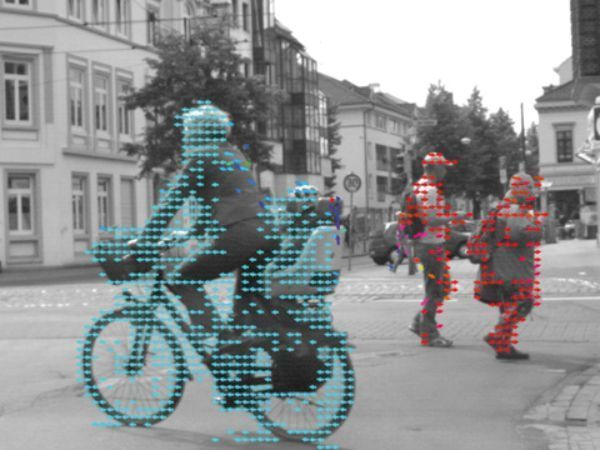
\includegraphics[width=0.8\linewidth]{Figures/opticalflow.jpeg}
 \caption{Motion Vector in Video Codec.}
 \label{fig:opticalflow}
\end{figure*}
\begin{figure*}
\centering
 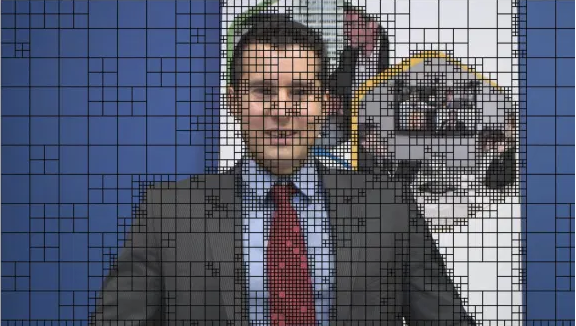
\includegraphics[width=0.8\linewidth]{Figures/macroblock.png}
 \caption{Macroblock in Video Encoder.}
 \label{fig:macroblock}
\end{figure*}
Figure \ref{fig:opticalflow} shows the optical flow (or motion vector) field of an image. Look at the objects in the image above and the motion vectors drawn on them. By analyzing the motion vectors, it is clear that a bicycle is moving towards the left side while two pedestrians are moving towards the right side. The speed of their motion is categorized by the magnitude of the motion vectors and their direction by the angel of the motion vectors. And therefore, it is necessary to send the motion vector for every pixel to the video decoder.\\
 In video coding standard, motion compensation is a practical method of motion compensate for movement of blocks of the current frame. The current frame is sub-devided in MxN blocks called macroblocks as shown in Figure \ref{fig:macroblock}. The following steps are carried out for each block MxN samples in the current frame:
\begin{itemize}
\item “Searching an area in the reference frame (past or future frame) to look after a 'matching' MxN-sample region. This process is to find the best match and is known as motion estimation”.
\item “The selected candidatge region becomes the predictor for the current MxN block and is removed from the current block to form a residual MxN block (known as motion compensation)”.
\item “The residual block and the offset between the current block and the position of the candidate region (motion vector) is encoded and transmited”. 
\end{itemize}
\begin{figure*}
\centering
 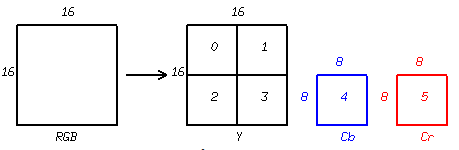
\includegraphics[width=0.8\linewidth]{Figures/yuv420.png}
 \caption{Macroblock (4:2:0).}
 \label{fig:yuv420}
\end{figure*}
	In H264/AVC standard, the macroblock, coressponding to a block size of 16x16 pixel is the basic unit for motion compensated prediction. In the RGB colour space, each pixel is represented by three numbers indicating the relative proportions of Red, Green and Blue. However, human eyes are more sensitive to luminance ( brightness ) than to colour. Thus, data can be down sample by transforming the RGB to YCbCr which throw some color components without causing much visual distortion. In example, in the 4:2:0 sampling format, Y has double Cb and Cr each has half the horizontal and vertical resolution of Cb and cr. Figure \ref{fig:yuv420} shows YCbCr 4:2:0 format with a 16x16 pixel macroblock. The macroblock is divided into 8x8 sample blocks. In the RGB space, a macroblock has a total of 3x4 = 12 (8x8 sample blocks) ( four for each of the colors Red, Green and Blue ). However, there are only six sample blocks in YCbCr 4:2:0 format, four for the Y component and 1 for each of Cb and Cr component.\\
  In  motion compensation, the MVs of other neighboring blocks in the current frame or in the earlier coded frames \cite{laroche2008rd}, \cite{jiang2019spatial} are correlated with MV of a current block. While intra-picture prediction uses correlations between spatially neighboring samples, then inter-picture prediction makes use of temporal correlation between frames to derive a motion-compensated prediction (MCP) for a block of frame samples \cite{bross2014inter}.
\begin{figure*}
\centering
 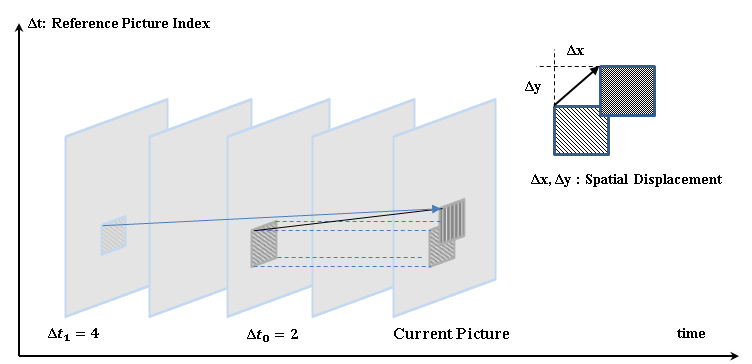
\includegraphics[width=1.0\linewidth]{Figures/mv.png}
 \caption{ The eeference MV model in video coding.}
 \label{fig:mv}
\end{figure*}
For intra-prediction, we assume that neighboring blocks possibly correspond to the same moving object with similar motion and that motion  is continuous to change over time. As the result, using MV in neighboring blocks as predictor can reduce the size of the signaled motion vector difference. For this block-based MCP, a video frame is divided into rectangular blocks. Figure \ref{fig:mv} presents the novel concept of MCP with a translational motion model. Using this model, the position of the block in a previously decoded picture is represented by a motion vector $(\Delta x, \Delta y)$, where $\Delta x$ is the horizontal and $\Delta y$ the vertical displacement relative to the position of the current block. These motion vectors are coded by entropy coding and placed into a compressed bitstream to send to the video decoder side,  and the decoder will use these MVs, along with one or more previously decoded pictures, to reconstruct the current image. On the other hand, in H.264/AVC, each video sequence is devided into groups of pictures (GOP), comprising at least one intra code I frame, uni-directionally predicted P frames and bi-directionally predicted B frames. Normally, the first frame in a GOP is intra coded I frame and follows by P, B frames. I frame utilize raw data from camera, while other frames in a GOP use the predictive coding involved motion vectors displacement. \\
%This is done by finding a displacement vector, i.e motion vector, for each block so that it optimises the rate-distortion requirements. As a result of the search criteria for 
\section{Compressed-Domain Based Moving Object Detection Using Motion Vector}
% Uncomment this line, when you have siunitx package loaded.
%The SI Units for dynamic viscosity is \si{\newton\second\per\metre\squared}.
%I'm going to randomly include a picture Figure~\ref{fig:minion}.


%If you have trouble viewing this document contact Krishna at: \href{mailto:kks32@cam.ac.uk}{kks32@cam.ac.uk} or raise an issue at \url{https://github.com/kks32/phd-thesis-template/}


%\begin{figure}[htbp!] 
%\centering    
%
\includegraphics[width=1.0\textwidth]{minion}
%\caption[Minion]{This is just a long figure caption for the minion in Despicable Me from Pixar}
%\label{fig:minion}
%\end{figure}
 As mentioned in last section, MVs are extracted for each motion block between the current and referenece frames. By minimising the prediction residual, the MVs present the temporal displacement between the two block in the process of motion compression. As the result, MV information will follow the real motion of objects and can be used for tracking purpose.\\
In recent researches, the compressed-domain based video analytics methods such as: \cite{bombardelli2018efficient},\cite{khatoonabadi2012video}. they are based on video coding features such as MVs, macroblock partition, and quantization coefficients, have been proposed. In \cite{bombardelli2018efficient}, the authors applied a probabilistic technique of computer vision for image separation, known as Graph Cut \cite{boykov2001fast}, modeling with MVs rather than pixels and adapted to the additional temporal dimension of video signals. “Using MVs and a spatio-temporal Markov random field (ST-MRF) model that naturally integrates the spatial and temporal aspects of the object’s motion for tracking. In general, these approaches do not rely on pixels and studies by only using the codec’s MVs and block coding modes extracted bitstream through inexpensive partial decoding. In this manner, computing and storage requirements have been significantly reduced compared to pixel-domain” (Nguyen Van Dien and Jaehyuk Choi, 2020, p.4).\\

\begin{figure*}
\centering
\subfloat[]
{
    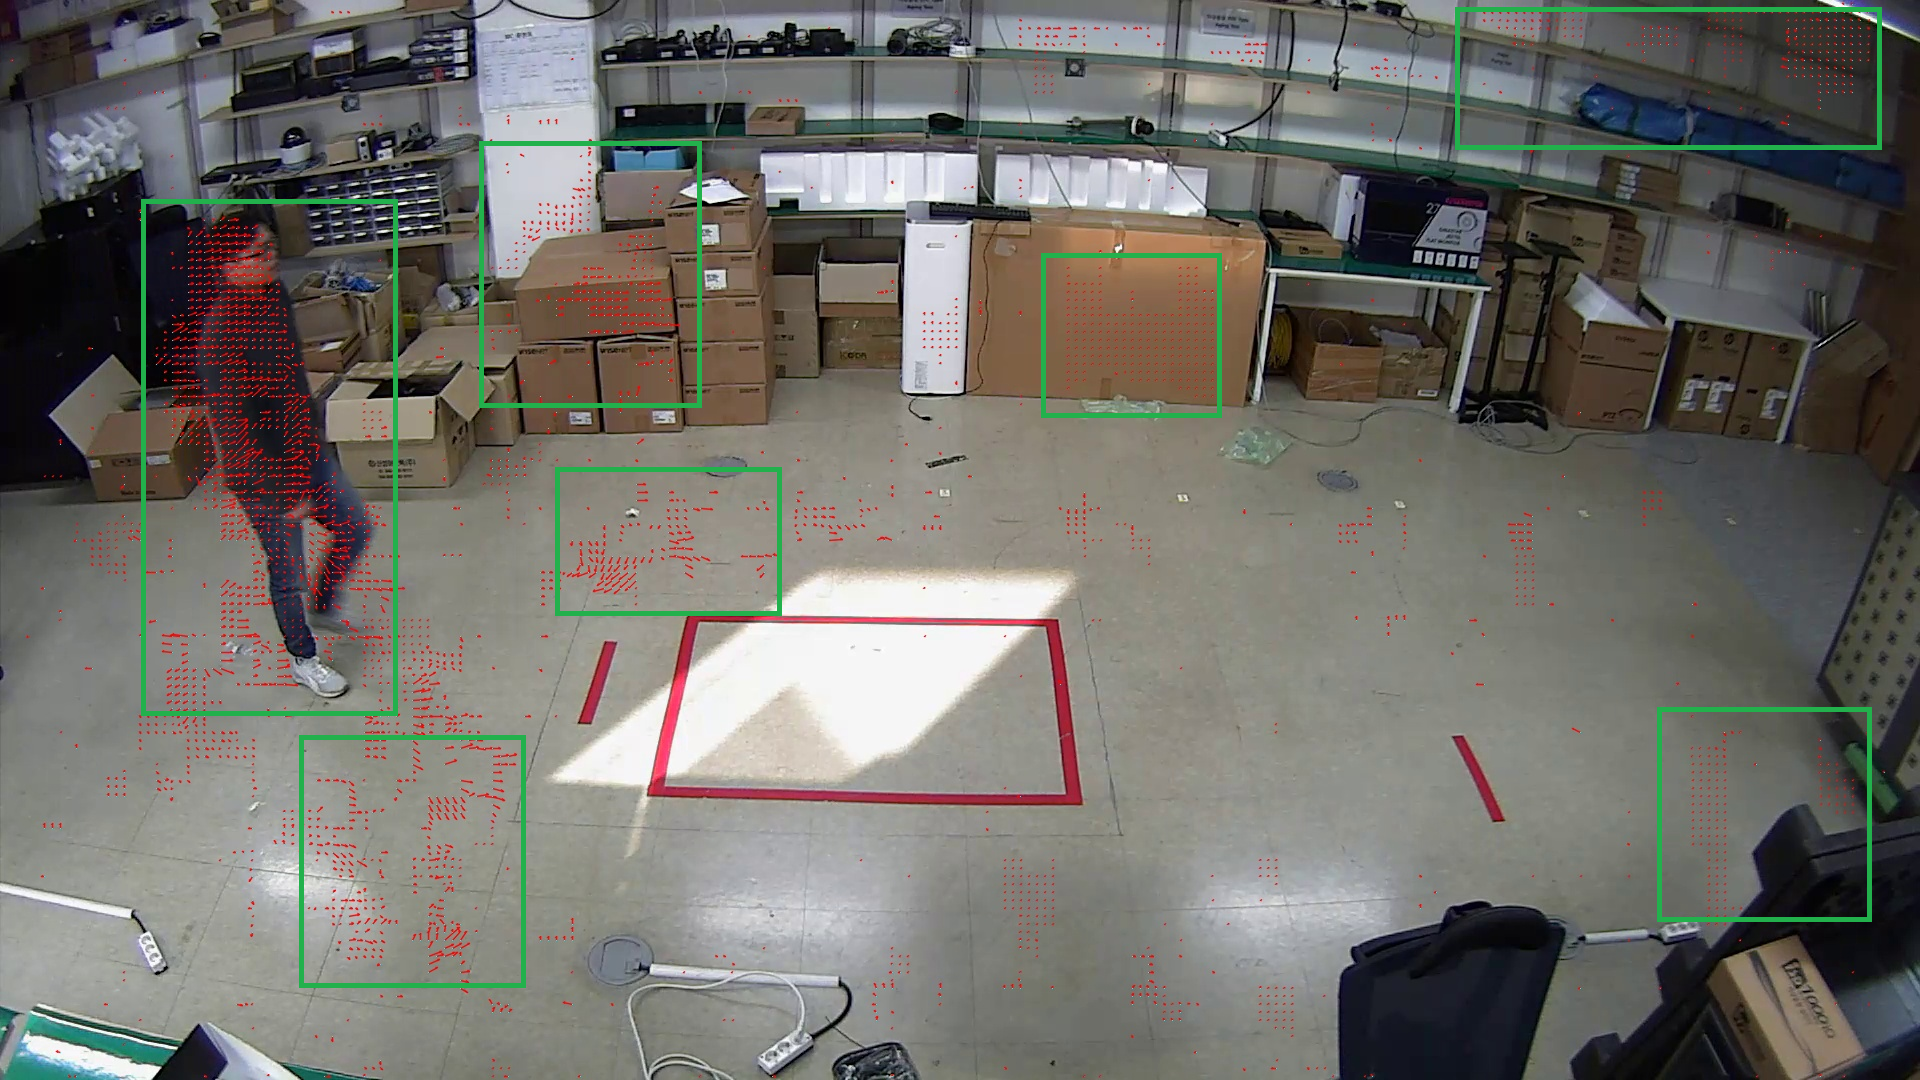
\includegraphics[width=0.5\linewidth]{Figures/noise.png}
}
\subfloat[]
{
    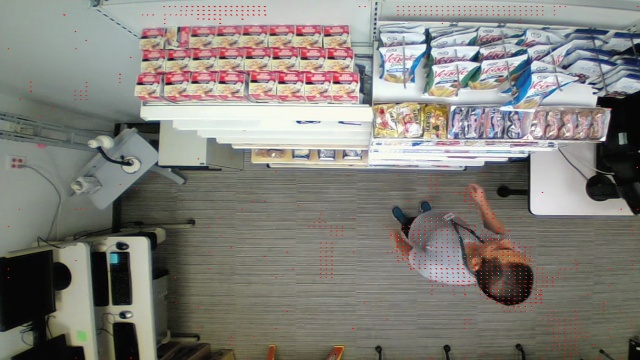
\includegraphics[width=0.5\linewidth]{Figures/156_mv_0.jpg}
}\\
\subfloat[]
{
    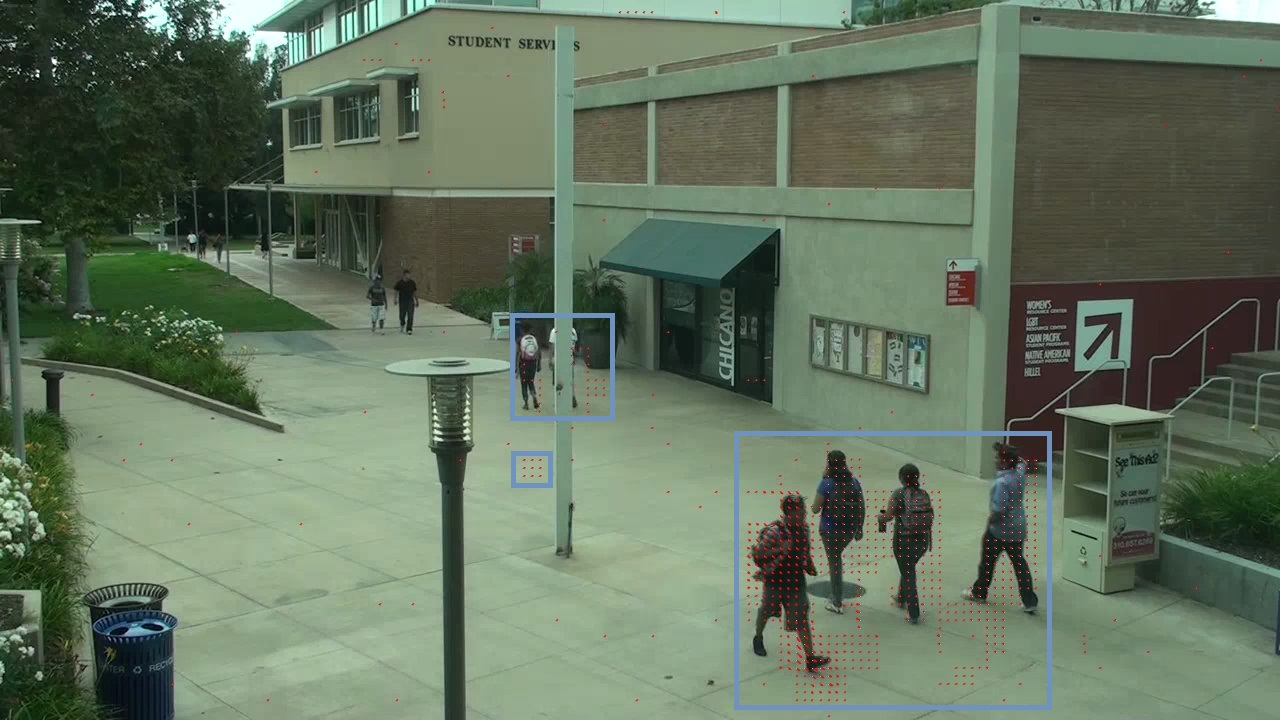
\includegraphics[width=0.5\linewidth]{Figures/3.jpg}
}
\subfloat[]
{
    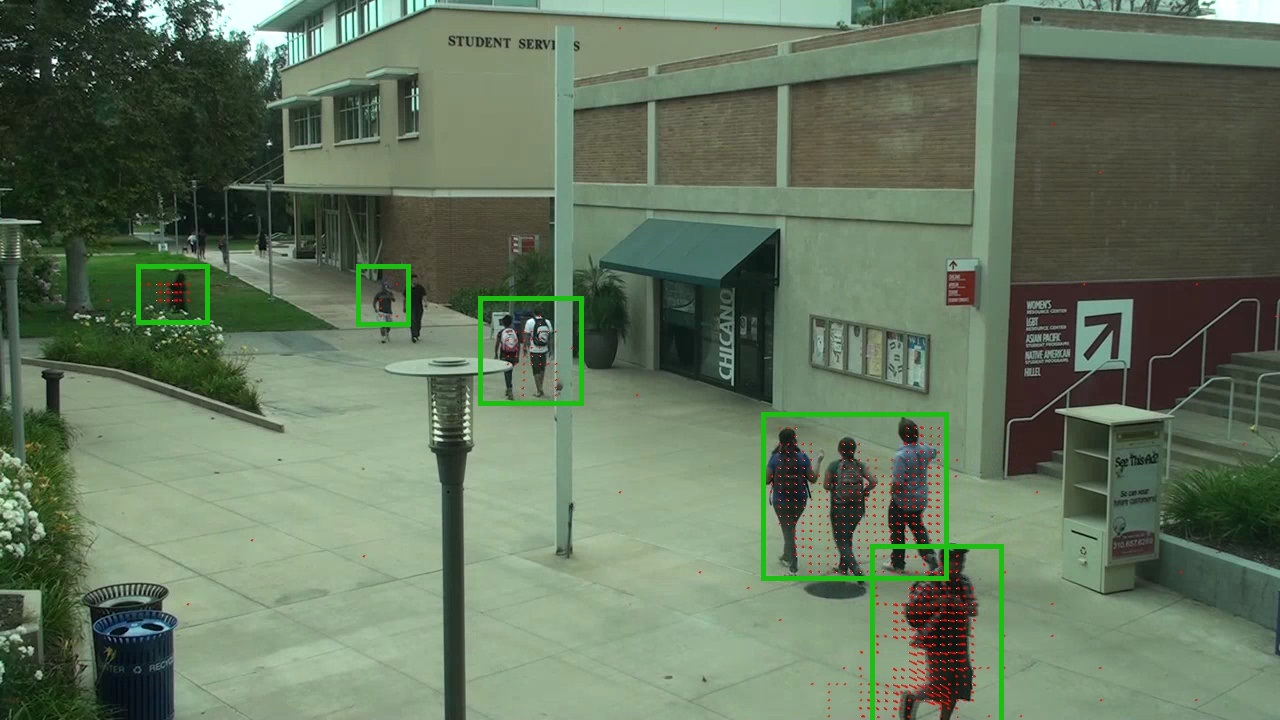
\includegraphics[width=0.5\linewidth]{Figures/34.jpg}
}
 \caption{ The example of MV extraction.(a) Test video sequence from recorded camera, (b, c, d) Test video sequence from VIRAT dataset.}
 \label{fig:noise}
\end{figure*}

The primary limitation of this approach is that it may lead to a noisy MV field that does not necessarily correspond with actual object movement of the object in the scene, as shown in Figure \ref{fig:noise}. “The noisy MVs fail to provide useful information such as those attributed to illumination changes and background movement. The amount of noise MVs is relatively reduced compared to the correctly estimated MVs because noisy vectors are continuous and similar MVs from real moving objects. Another challenge of this approach is the lack of information about the object’s appearance such as color, edges and texture, because these features would require complete decoding of the compressed bitstream. In this study, our aim is to work in the compressed domain and uses only the MVs from the compressed bitstream to detect and track moving objects in video frames” (Nguyen Van Dien and Jaehyuk Choi, 2020, p.4).
%To apply the IoU-based object tracking algorithm \cite{rezatofighi2019generalized}, MVs are clustered into blobs and simply represented with object bounding boxes.

\section{Pixels-Domain Based Moving Object Detection using Deep Learning}
Because of more reliable features that can be extracted from the pixel data, the majority of moving object detections have been done in pixel domain, even it requires full decoding the video stream. In pixels domain, a VA server analyzes the R-G-B image to find the appearance objects and spatial events. The drawback and exciting research problem, and it is overcome by the recent advantages of hardware and deep learning \cite{zeng2018background},\cite{chen2017pixel},\cite{babaee2018deep},\cite{wang2017interactive},\cite{patil2018msfgnet},\cite{ou2019moving}. There are two main methods that are considered for moving object detection in pixels domain.
\subsection{The combination of background modeling and CNN based object classification}
\begin{figure*}
\centering
\subfloat[]
{
    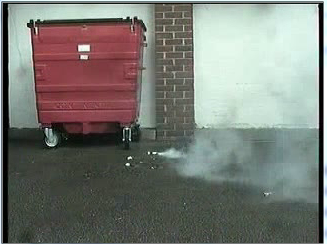
\includegraphics[scale=0.5]{Figures/input_img.png}
}
\subfloat[]
{
    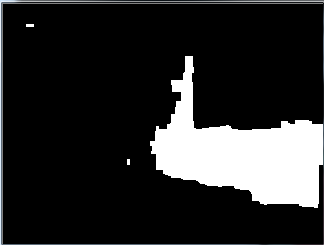
\includegraphics[scale=0.5]{Figures/fg_subtration.png}
}\\
\subfloat[]
{
    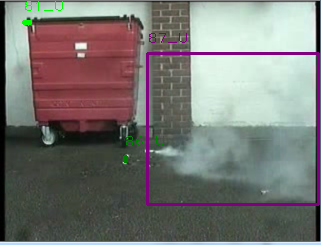
\includegraphics[scale=0.5]{Figures/blob_detection.png}
}
\subfloat[]
{
    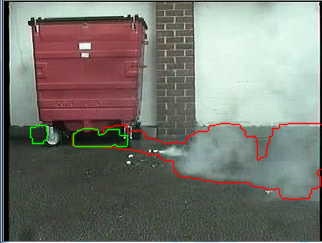
\includegraphics[scale=0.5]{Figures/smoke_region.png}
}
\caption{Smoke detection pipeline: (a) input frame, (b) the foreground subtraction, (c) the blob detection, (d) the smoke candidates classification }
\label{fig:bgmethod}
\end{figure*}
\begin{figure*}
\centering
 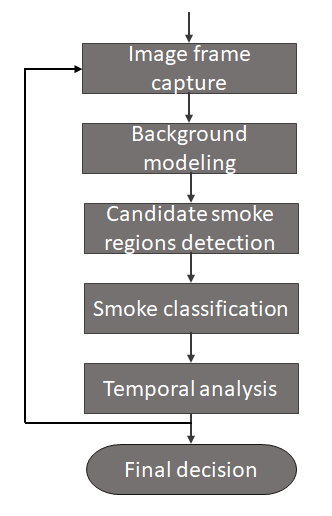
\includegraphics[width=0.3\linewidth]{Figures/smoke.jpg}
 \caption{The pipeline of video- based smoke detection algorithm.}
 \label{fig:smoke}
\end{figure*}
The background subtraction approach \cite{lee2012adaptive}\cite{stauffer1999adaptive} subtracts the current image and background image to eliminate the background, and then detects moving targets based on pixel clustering. This method is widely used for object detection. There are many methods that have been purposed for building the background model, e.g.  \cite{lu2008improved} presented a novel real-time motion detection method that integrates the temporal differencing, double background filtering, optical flow, and morphological processing methods to obtain excellent performance. Moreover, the authors of \cite{stauffer1999adaptive} discussed modeling each pixel as a grouping of Gaussians using an on-line approximation to renew the model. “The Gaussian distributions of the adaptive mixture model were then assessed to determine which model can be presumed to be obtained from a background process. This method’s advantage is its simple implementation, low computational resource requirements, robustness in the presence of environmental noise, and dynamic background. However, it has limitations with shadows, background changes, as well as object localization and classification. Furthermore, object detection based on the background model cannot detect the individual objects in a group or a block object. In general, the aim of background subtraction is to separate foreground images from background ones in the form of blobs, followed by an object classification process” (Nguyen Van Dien and Jaehyuk Choi, 2020, p.5). The detected blobs then help classify each blob into subclasses, as shown in Figure \ref{fig:bgmethod}, which shows the complete process of this approach is to perform smoke detection with the detail of flow-char is drawn in Figure \ref{fig:smoke}. In this example, smoke classification was done by trained convolutional neural networks (CNN) model which was described in \cite{krizhevsky2017imagenet} for image classification. This a relatively new approach in machine learning, which ultilize CNNs to achive the very accurate classification of images. \cite{lecun2010convolutional}\cite{jarrett2009best}\cite{lee2009convolutional}. 
\begin{figure*}
\centering
 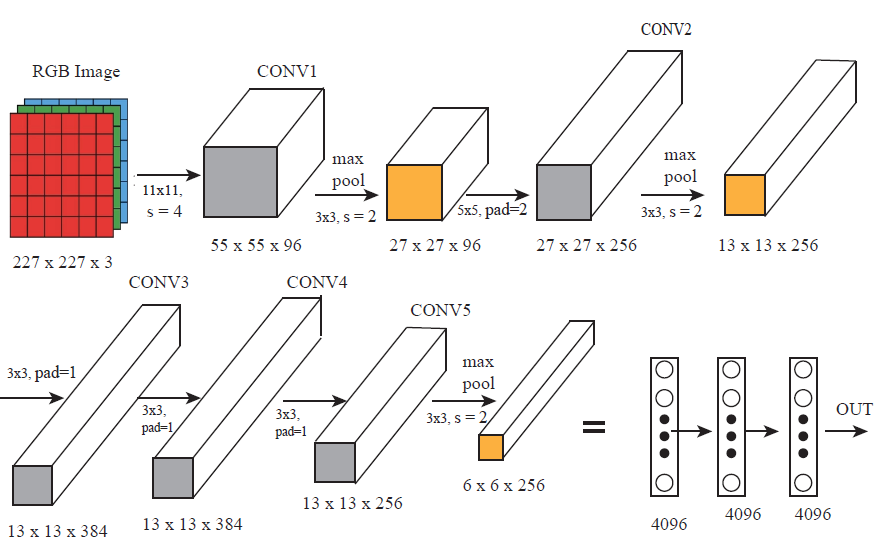
\includegraphics[width=0.8\linewidth]{Figures/AlexNet.png}
 \caption{Architecture of the Alexnet CNN model.}
 \label{fig:alex}
\end{figure*}
Figure \ref{fig:alex} shows the original architecture of the trained model, first five layer are convolutional and some of them are followed by max pooling layer. The next are three fully-connected layer, the last fully-connected layer computes class score of trained class labels.

The accuracy of CNN based model can be changed by varying their depth and breadth. For example, by combining CNN and transfer learning, the authors of \cite{hussain2018study} achieved an average accuracy of 70.1\% using the CIFAR-10 \cite{krizhevsky2009learning} dataset.

\subsection{Deep Learning based Moving Object Detection}
\label{subsec:frameworks}
\begin{figure*}
\centering
\subfloat[]
{
    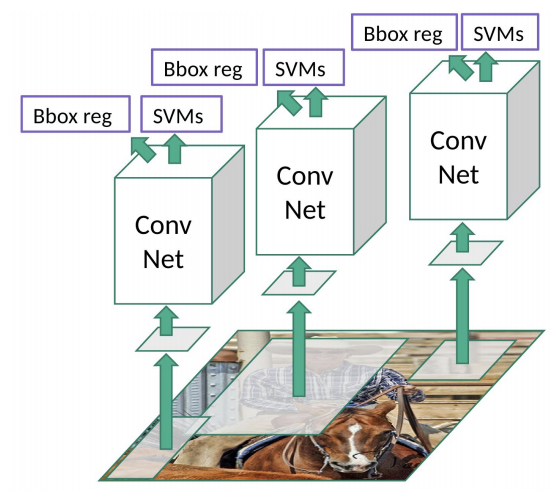
\includegraphics[scale=0.3]{Figures/rcnn.png}
}
\subfloat[]
{
    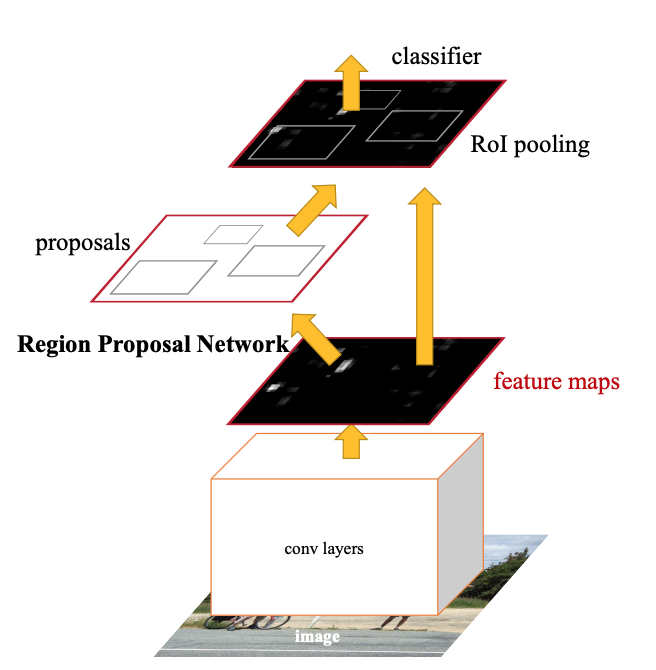
\includegraphics[scale=0.45]{Figures/faster_rcnn.png}
}\\
\subfloat[]
{
    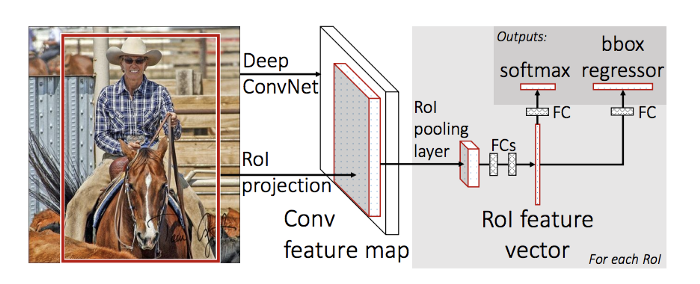
\includegraphics[scale=0.5]{Figures/fast_rcnn.png}
}
\caption{CNN based Object Detection Framework Structure.(a) RCNN, (b) Faster-RCNN, (c)Fast-RCNN.}
 \label{fig:cnn}
\end{figure*}

\begin{figure*}
\centering
 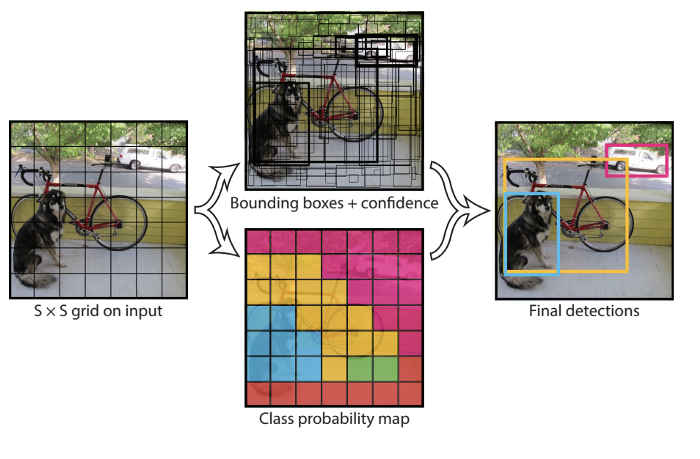
\includegraphics[width=0.8\linewidth]{Figures/yolo.png}
 \caption{YOLO Structer.}
 \label{fig:yolo}
\end{figure*}

Hybrid background subtraction and deep learning classification enhance the system’s accuracy; “however, there are issues with detection of individual objects in a group or blocked objects and the background changes by the lighting condition and the environmental noise” (Nguyen Van Dien and Jaehyuk Choi, 2020, p.5). Hence, the usage of deep learning is considered for robust object detection tasks. We have identified three primary object detection methods using deep learning:
\begin{itemize}
\item R-CNN model, Fast R-CNN model, Faster R-CNN model.
\item You Only Look Once (YOLO)
\item Single Shot Detectors (SSDs) 
\end{itemize}
“R-CNN \cite{girshick2014rich} uses selective search \cite{uijlings2013selective} to extract several regions, called region proposals, from the image; it then attempts to classify a large number of regions. Each region proposal is placed into CNNs to extract features, which are fed to a support vector machine to classify the presence of object within the candidate region proposal as shown in Figure \ref{fig:cnn}(a). The limitation of this method is that it requires a large amount of time to train and deploy networks because it has to classify multiple region proposals per image. Fast R-CNN \cite{girshick2015fast} solves the limitations of R-CNN by putting the entire image into the CNNs to generate a convolutional feature map and identify the region of proposals based on the map, thus reducing the number of classified region of proposals as drawn in Figure \ref{fig:cnn}(c). Both R-CNN and Fast R-CNN use selective search to identify the region proposals. Selective search is a slow and tedious process that affects the network’s performance. Faster R-CNN \cite{ren2015faster} was proposed to allow the network to learn the region proposals as shown in Figure \ref{fig:cnn}(b); it uses a separate network to predict the region proposals rather than use a selection search algorithm on the feature maps output using the CNN layer. YOLO \cite{redmon2016you} is an object detection system to detect object at real-time speed. Unlike R-CNN, Fast R-CNN and Faster R-CNN, which use regions to localize the object within the image, YOLO ultilize a single neural network to predict the bounding boxes and the class probabilities for these boxes during training and test periods. Hence, YOLO only examines the input picture once to predict the presence and location of objects. YOLO divides the input image into an SxS grid, and multiple bounding boxes can exist within each grid. For each bounding box, the network outputs a class probability and offset value for the bounding box” (Nguyen Van Dien and Jaehyuk Choi, 2020, p.7). The bounding boxes with class probabilities above a certain threshold value are then selected and used to locate the object within the image as shown in Figure \ref{fig:yolo}. “Specially, YOLOv3 network architecture has 24 convolutional layers, followed by two fully connected layers as shown in Figure \ref{fig:yolov3}. The initial convolutional layers of the network extract feature from the image, while the fully connected layers predict the output probabilities and coordinates. According to performance comparison in \cite{redmon2018yolov3}, YOLOv3 is faster (45 frames per second (FPS)) than the other object detection algorithms. Faster R-CNN is more accurate than YOLOv3 (a mean average precision (mAP) of 73.2, as compared to 63.4); however, YOLOv3 is considerably faster than Faster R-CNN (FPS of 45, as compared to 7). Therefore, SSDs  \cite{liu2016ssd} were released as a balance between these two methods. Compared to YOLO, an SSD runs an input image through a convolutional network only once and computes a feature map. Then, a small 3 × 3 sized convolutional kernels are run on this feature map to predict the bounding boxes and categorization probability. Moreover, SSD uses anchor boxes at various aspect ratios comparable to Faster-RCNN and learns the off-set to a certain extent compared to learning the box. The SSD is able to detect objects of multiple scales because every convolutional layer function at a diverse scale. Compared to the YOLOv3 method \cite{redmon2018yolov3}, the SSDs attain similar accuracy but run slower” (Nguyen Van Dien and Jaehyuk Choi, 2020, p.7). In this study, YOLOv3 was applied to robust human detection at cloud servers for our implementation. 

\begin{figure*}
\centering
 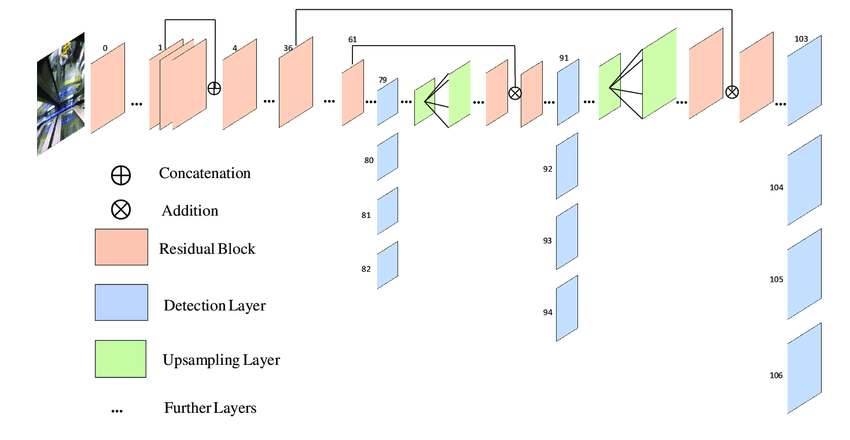
\includegraphics[width=1.0\linewidth]{Figures/yolov3.png}
 \caption{YOLOv3 Network Model.}
 \label{fig:yolov3}
\end{figure*}

%!TEX root = ../thesis.tex
%*******************************************************************************
%****************************** Third Chapter **********************************
%*******************************************************************************
%Here you make the strongest statement concerning observations. Highlight the information you want readers to remember. Explain how the results correlate with the problems you have indicated in the introduction. Describe all new things that are significant in finding a solution.

%The recommendations part is for giving advice and indicating other actions that will help to solve particular problems. Sound your own opinion about the direction of future research. Most of the time you have to write it. Just like a research proposal.

%Acknowledgments part is a paragraph where you mention everyone who helped you with composition. Place all cited and used information resources into one list or form an annotated bibliography if needed.
\chapter{Methodology}

% **************************** Define Graphics Path **************************
%\ifpdf
%    \graphicspath{{Chapter3/Figs/Raster/}{Chapter3/Figs/PDF/}{Chapter3/Figs/}}
%\else
%    \graphicspath{{Chapter3/Figs/Vector/}{Chapter3/Figs/}}
%\fi
In this section, the proposed edge-to-cloud system for surveillance video analytics applications is presented detaily. And then, the method for moving objects detection in compressed-domain is analyzed. In addtion, the performance evaluated model for video analytics platform is introduced. 

\section{The Edge-to-clound System Model for Surveillance Camera based Applications}
\begin{figure*}
\centering
 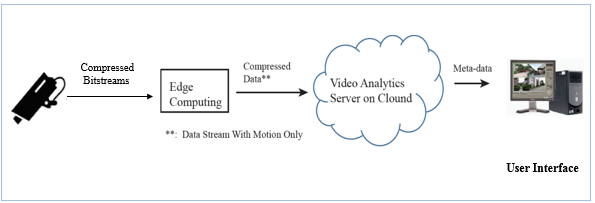
\includegraphics[width=1.0\linewidth]{Figures/arch.png}
 \caption{ Overview of the proposed edge-to-cloud system model.}
 \label{fig:arch}
\end{figure*}
There is a trend to forward computation from the network core to the edge where most of the data are generated. Edge computing has exhibited its potential in reducing the reaction time, minimizing bandwidth usage, and improving energy efficiency. Edge computing performs data processing at the “edge” of the network, close to the data source. For network cameras, audio and other sensors, there is a need to balance both cloud computing and edge computing domains to deliver refined, reliable, and usable data. For edge computing of delay-sensitive video tasks, a camera source node can offload its video task to nearby edge nodes via local wireless/optical networks and edge nodes are within the local communication range of the camera. The camera captures the video sequences and divides each of them into multiple video chunks, compresses these video chunks, and then delivers them to edge nodes. Next, edge nodes implement video processing functions on the received video chunks and upload the results to a cloud server for video analysis (such as object/event detection). A delay-sensitive video assignment is supposed to be processed within a limit and will fail if the deadline is passed. In this study, as shown in Figure \ref{fig:arch}, we consider an edge computing network, which comprises three primary components, namely, camera source node, edge node, and cloud server.
\begin{itemize}
\item Camera source node: the camera node periodically generates video tasks, divides each video task into a number of videos chunks, compresses video chunks at certain compression ratios, and then assigns compressed video chunks among all edge nodes as per scheduling policies.
\item Edge node: the edge has computational ability and storage capacity and helps preprocess video chunks. Moreover, edge nodes can form cooperative groups based on specific group formation policy and receive compressed video chunks as per the video load assignment policy.
\item Cloud Server: cloud server collects the preprocessing results from edge nodes, which has abundant computational abilities, and performs additional video analysis.
\end{itemize}
During a sparse edge node deployment, an edge node will only connect to one of the available cameras at a certain location; however, in a dense deployment, an edge node may have multiple choices on selecting multiple cameras. In this study, we focus on reducing processing load on cloud server by minimizing the video chunks that are fed from camera sources. Therefore, an edge device runs preprocessing tasks to filter uninteresting video chunks. The term “uninteresting video chunks“ is defined via scenario specification: for surveillance scenarios, it is static scenes without any objects and gradual changes.

\section{The Light-weight Runtime Moving Object Detection in Video Compressed Domain}
\begin{figure*}
\centering
 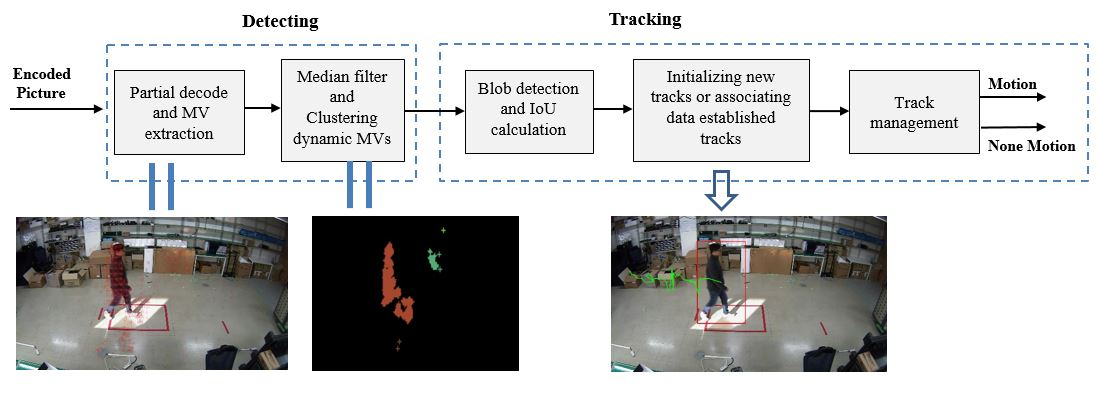
\includegraphics[width=1.0\linewidth]{Figures/arch.jpg}
 \caption{Workflow of the proposed detection-based tracking approach in compressed domain.}
 \label{fig:proposedMethod}
\end{figure*}
\begin{figure*}
\centering
\subfloat[]
{
    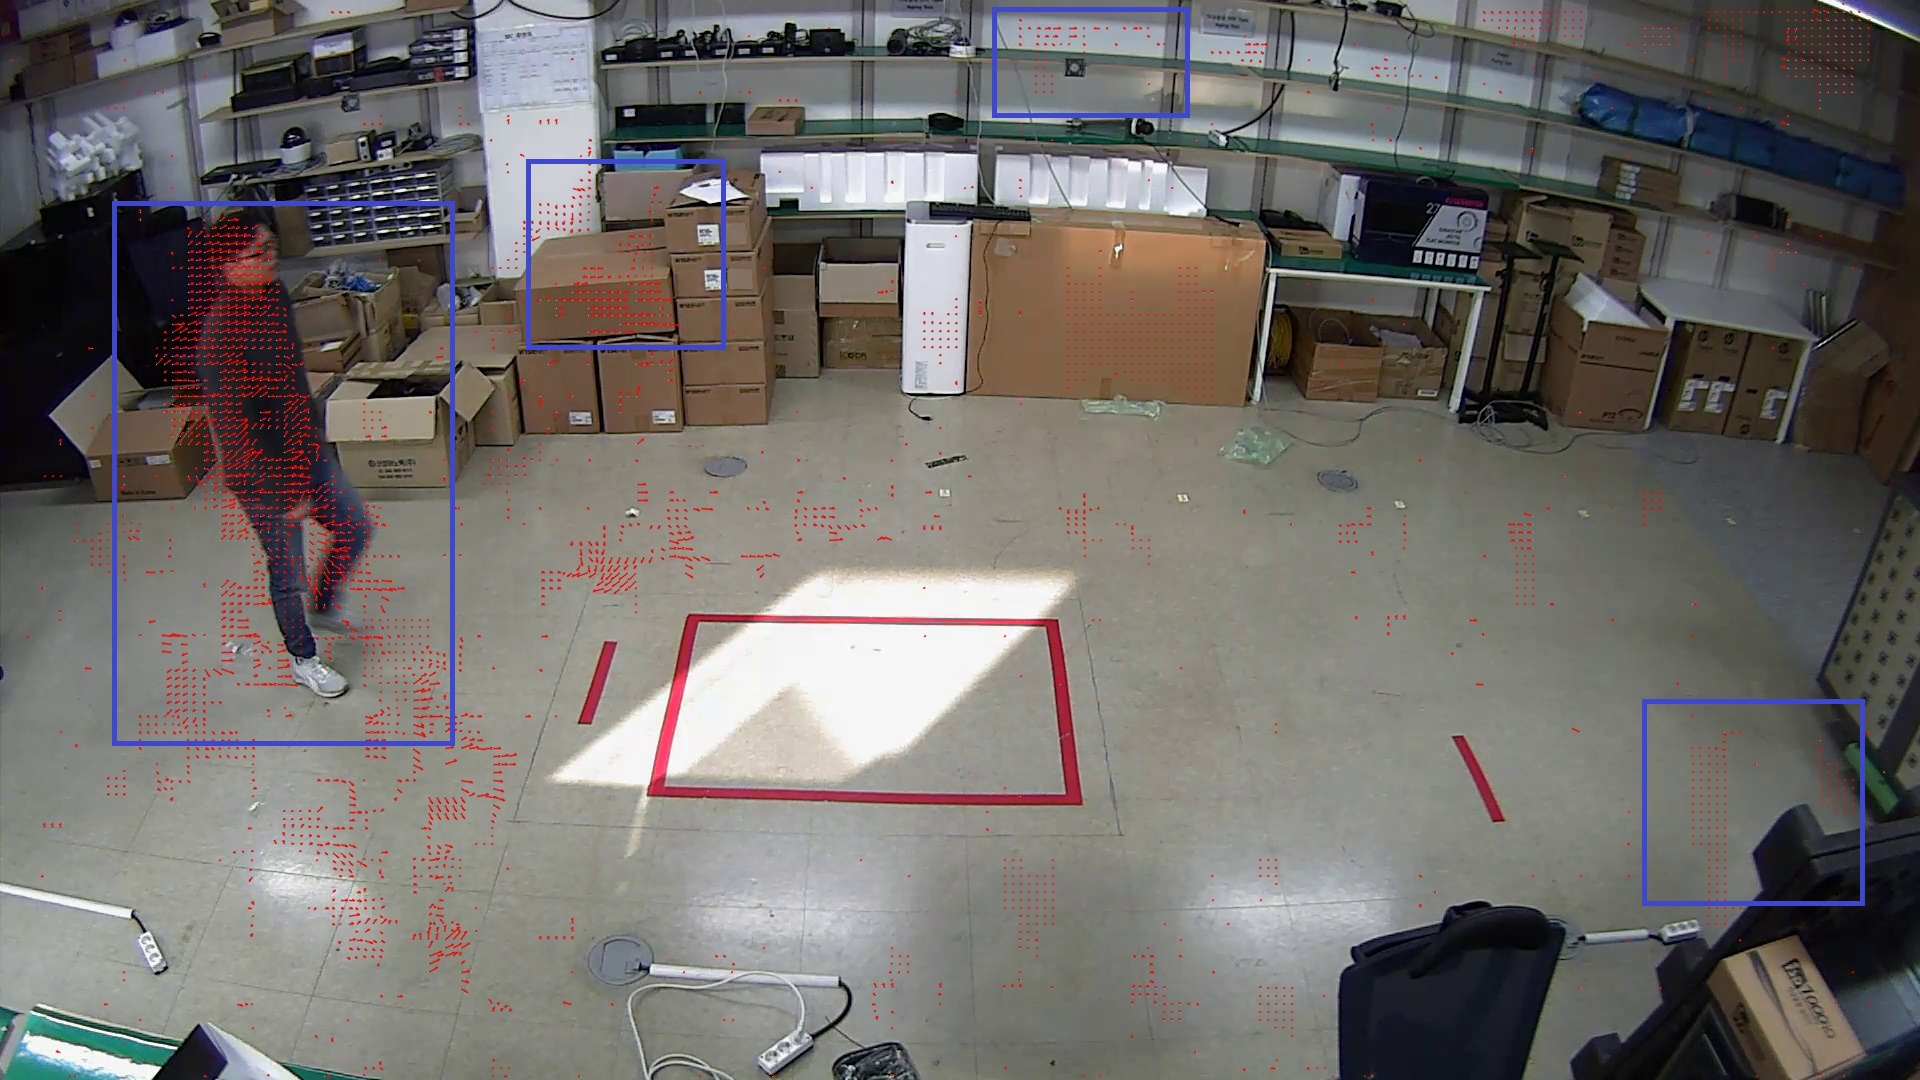
\includegraphics[width=0.3\linewidth]{Figures/1340.jpg}
}
\subfloat[]
{
    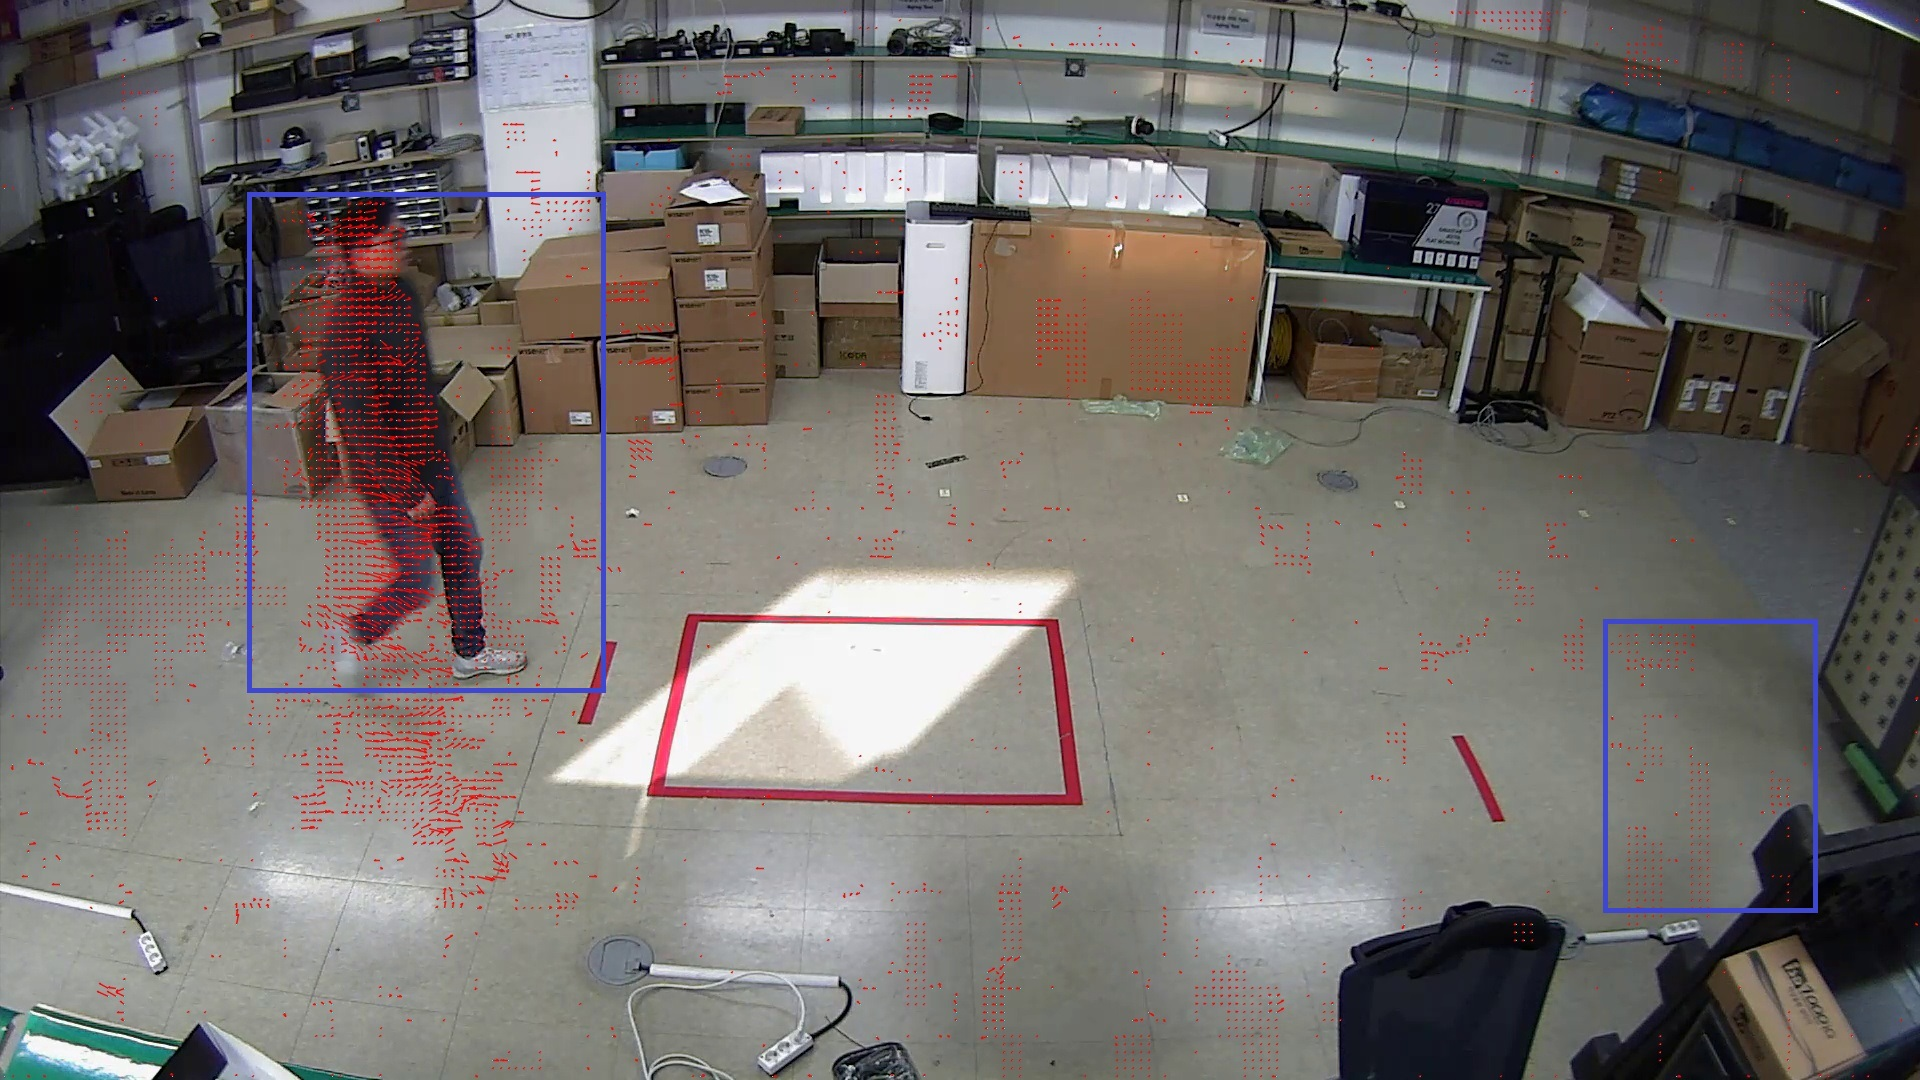
\includegraphics[width=0.3\linewidth]{Figures/1350.jpg}
}
\subfloat[]
{
    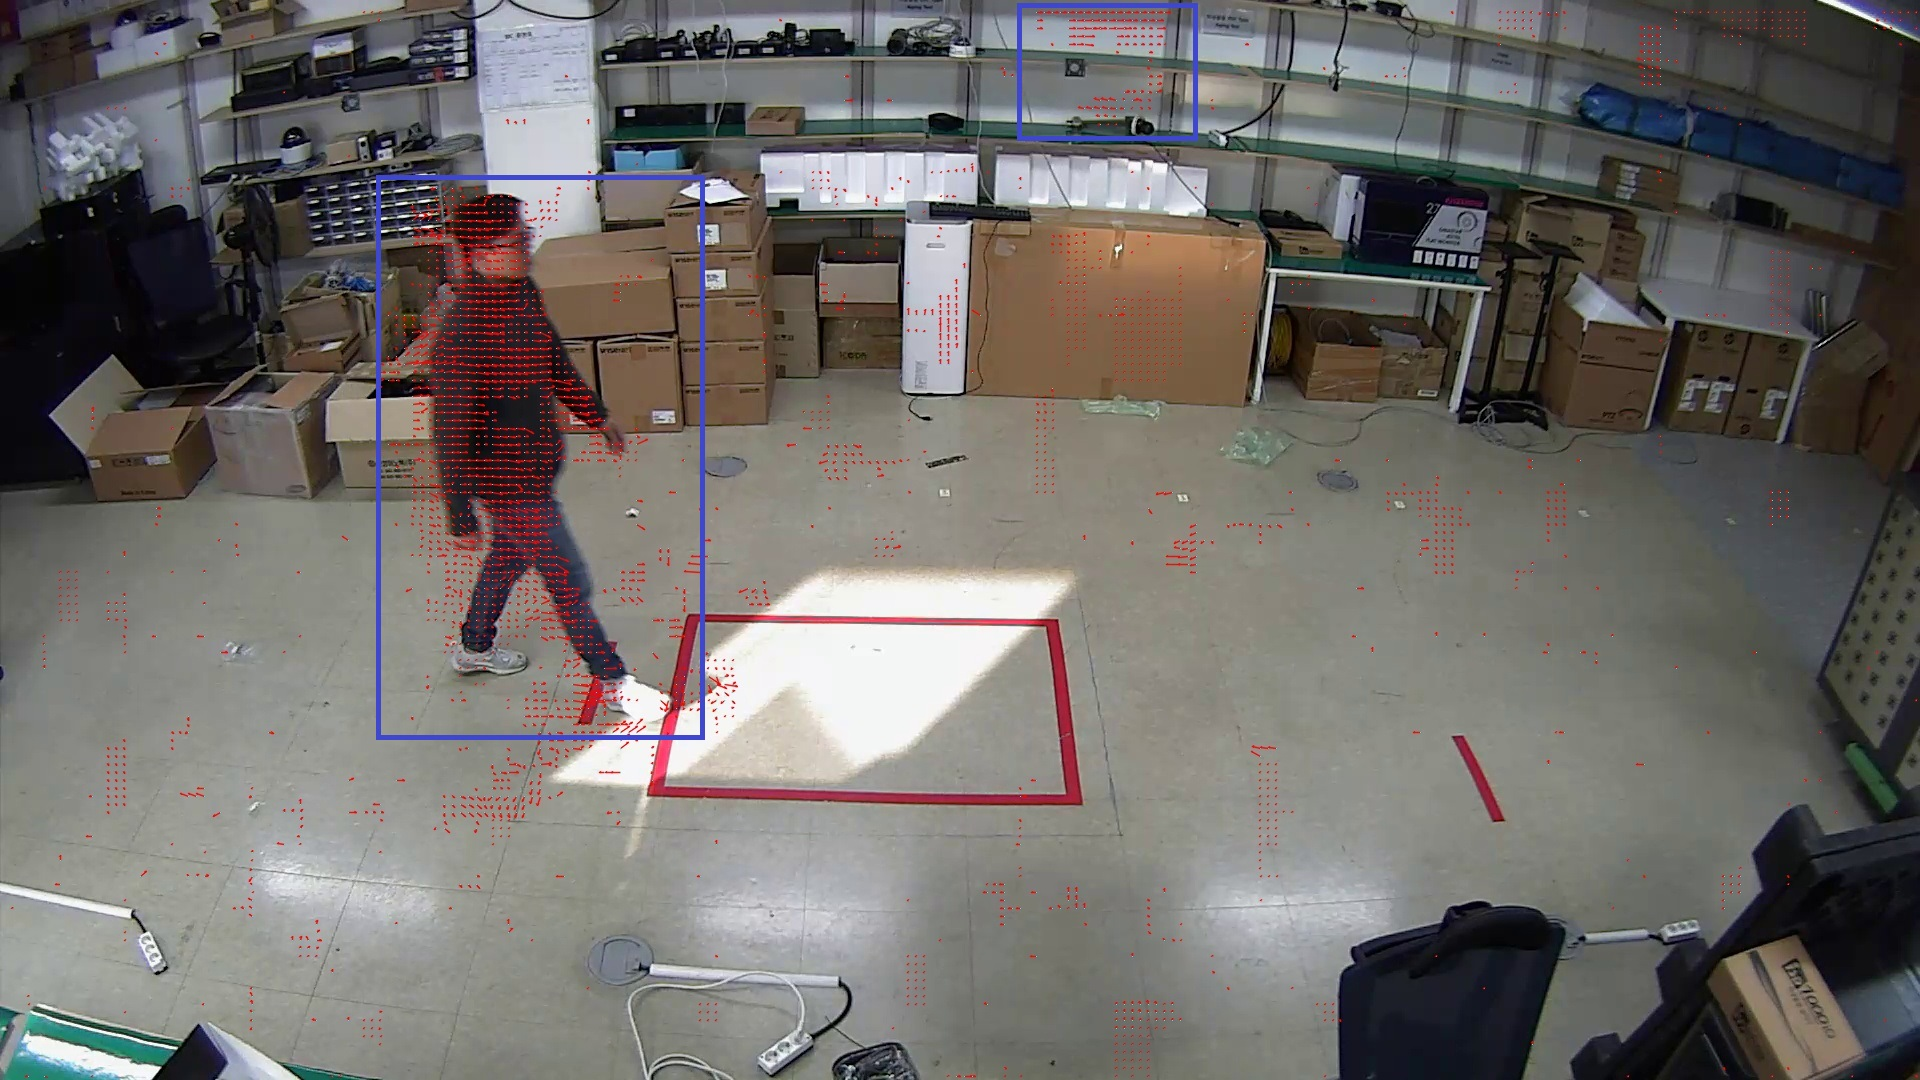
\includegraphics[width=0.3\linewidth]{Figures/1360.jpg}
}\\
\subfloat[]
{
    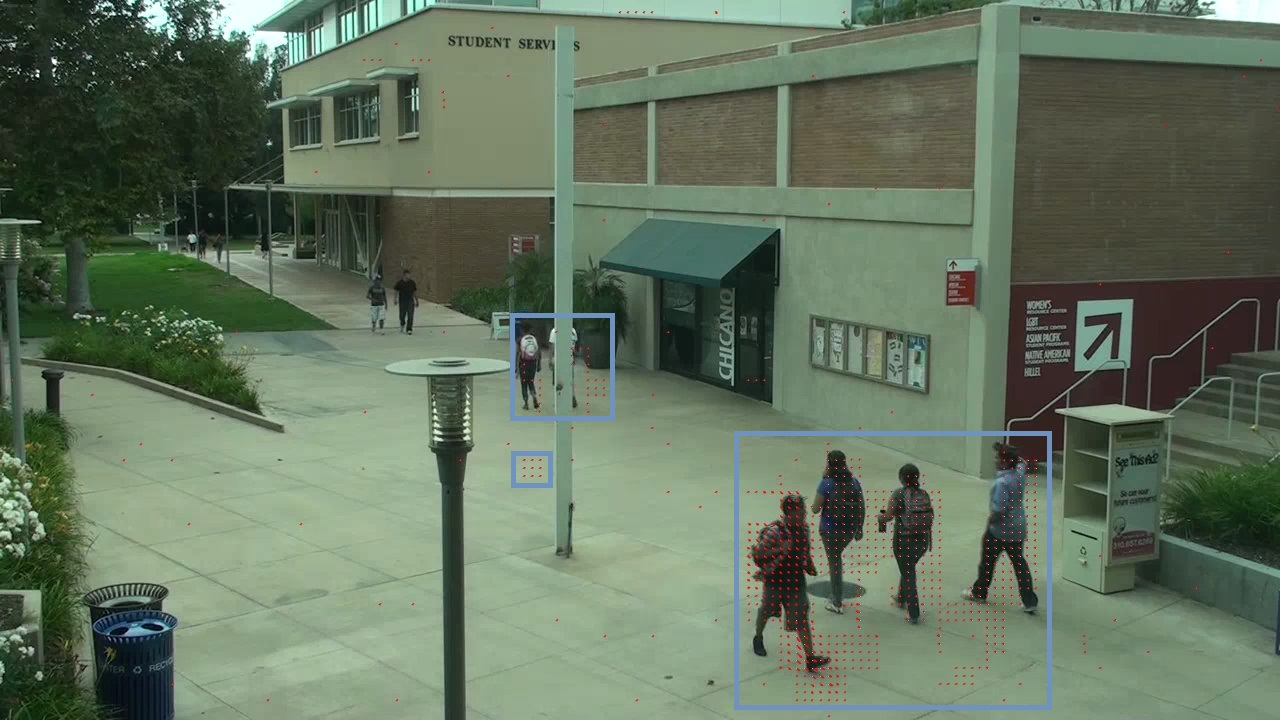
\includegraphics[width=0.3\linewidth]{Figures/3.jpg}
}
\subfloat[]
{
    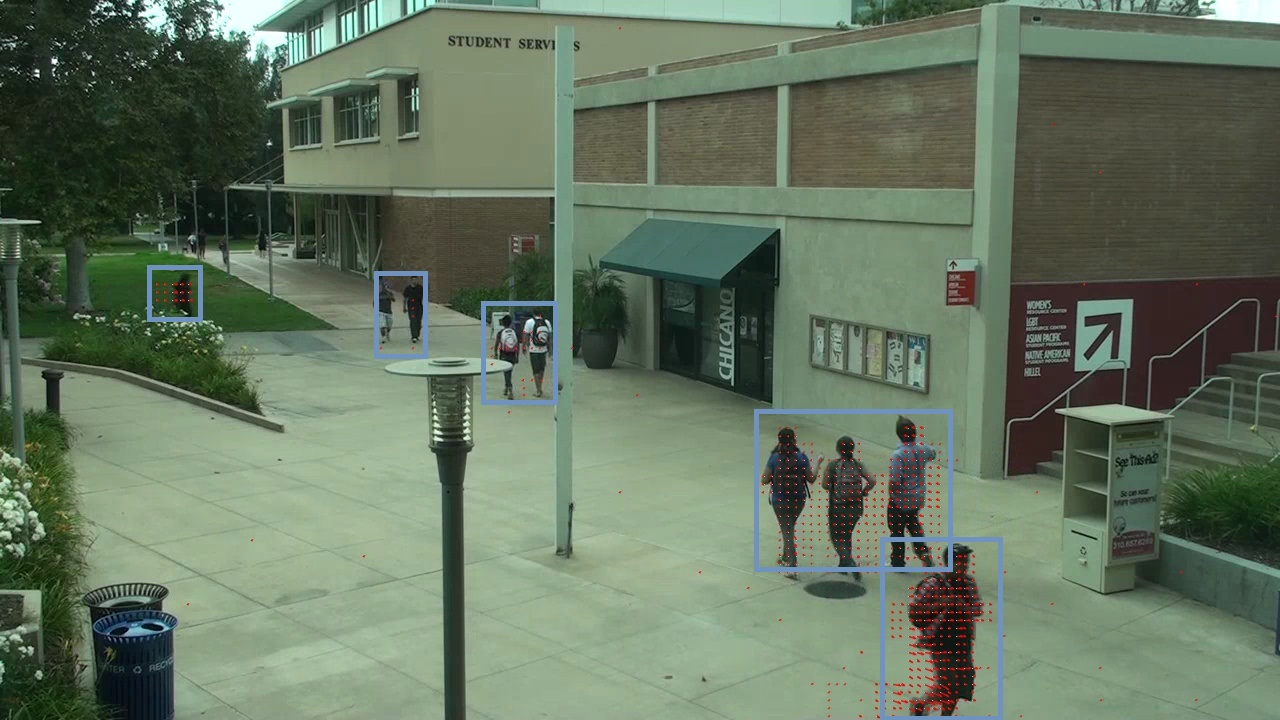
\includegraphics[width=0.3\linewidth]{Figures/35.jpg}
}
\subfloat[]
{
    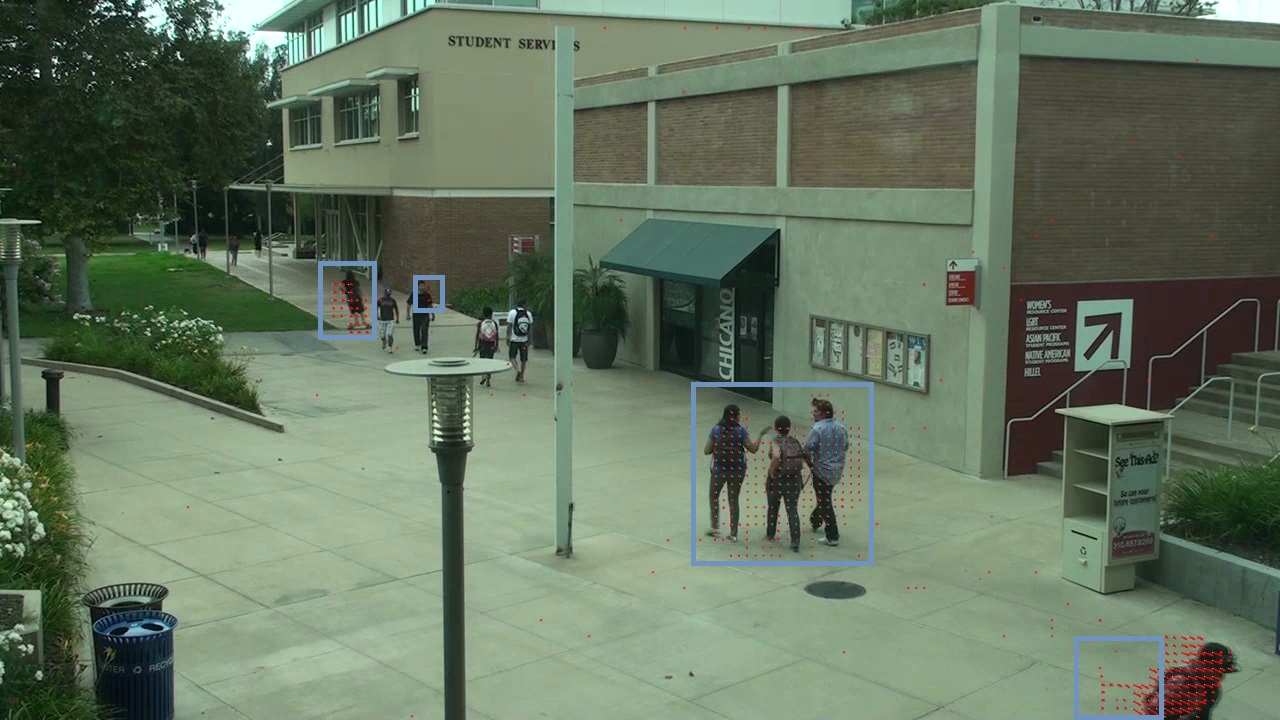
\includegraphics[width=0.3\linewidth]{Figures/70.jpg}
}
\caption{Video coding motion vector extraction from consecutive frames with two video test sequences.}
\label{fig:mvextract}
\end{figure*}
MV represents the changes between video frames may caused by:
\begin{itemize}
\item Object motion (car, human activity)
\item Camera motion (panning, tilt, zoom, rotation).
\item Lighting condition changes
\end{itemize}
The MV group generated by lighting change, usually randomly occur without following a certain flow and have various sizes. The MV group generated by human motion (walking, running),  move in certain direction and It’s size is similar with object size in video frame. This observation is good factor to classify MVs into real-motion and noise motion group. The aim of this method is to analyze only MVs at the edge device, recognize the real moving objects, and exclude the noised motions that are generated by environmental factors such as illumination changes and background movement, in the current video scene. For this purpose, we present a method that has a workflow shown in Figure \ref{fig:proposedMethod} to analyze the video coding MVs. In order to extract MVs from compressed bitstream, the input video stream is partially decoded and the collected MVs will include both real object MVs and noise MVs. The example of extracted MVs are represented in Figure \ref{fig:mvextract} in consecutive frames of two different video test sequences. To analyze these MVs, the following functionalities are involved.
\subsection{Median Filter and Moving Object Detection}
\label{sub:filter}
\begin{figure*}
\centering
\subfloat[]
{
    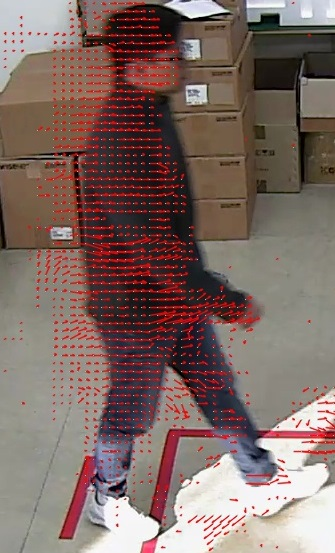
\includegraphics[scale=0.325]{Figures/1327_mv.jpg}
}
\subfloat[]
{
    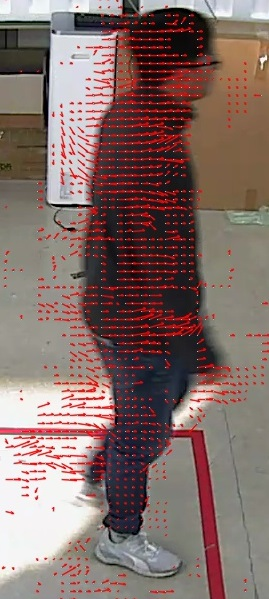
\includegraphics[scale=0.3]{Figures/1350_mv.jpg}
}
\subfloat[]
{
    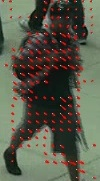
\includegraphics[scale=1.0]{Figures/30_mv.jpg}
}
\subfloat[]
{
    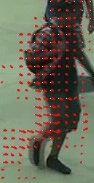
\includegraphics[scale=1.0]{Figures/10_mv.jpg}
}
\caption{Motion vector of a moving object in different video test sequences: (a, b) our record video, (c, d) Test video in VIRAT}
\label{fig:mvobject}
\end{figure*}
Compressed-domain MVs may not represent the actual of true motion due to the properties of motion estimation, biased towards efficient coding as shown in Figure \ref{fig:mvanalysis}(a,e). Therefore, it is desirable to eliminate motion vectors that can be categorised as unsuitable for moving objects detection. We assume that MVs  whose magnitudes are very high or very low, compared to the other MVs related to the moving object, has to be replaced with the median value of neighbouring MVs. Therefore, the application of vector median filter aims to reduce isolated vector noises and smoothen the difference of MV between adjacent blocks. Note that the sliding window approach is used for median filtering. Because H.264/AVC allows for variable-sized block partitioning, we construct a uniformly sample MV field by mapping all MVs to 4x4 blocks. Theoretically, the motion vector average (normalized vector) among all elements $N_{mv}$ in NxN (N=4 in this study) window function is calculated by Equation \ref{eqn:1}: 
\begin{equation}
\label{eqn:1}
N_{mv}= \frac{\sum_{i=1, j=1}^{N*N}MV_{ij}}{N*N}
\end{equation}          
Where: $MV_{ij}$ is the MV elements in the N×N window. Finally, the smoothened motion filter is presented, which is experimentally determined as shown in Figure \ref{fig:mvanalysis}(b,f) using the input MV, including isolated motion vectors noise, are smoothened in the areas that mostly correspond to the object boundaries. In order to detect the moving objects, a cluster detector is involved to determine the number of moving objects and their approximate positions in the scene. Then, a density-based cluster technique is applied to completely segment moving objects. The first step, MV whose magnitudes can be used to easily differentiate moving objects from the stationary background. However, it is difficult to directly and completely segment moving objects because not all MVs on the objects have the same motion state. While every part of a rigid body maintains nearly the same motion state, different parts of a non-rigid body can move in various ways (see Figure \ref{fig:mvobject}). In order to cluster detected MVs into dynamic clusters, a range search algorithm based on the euclidean distance of the MV point is used, under the presumption that dense points represents the same object. It requires a parameter $\varepsilon$ where $\varepsilon$ is the spatial distance threshold between density reachable MV. The goal is to partition \textit{n} MV points $\chi \subset \mathbb{R}^{d}$ into \textit{k} clusters using k-means filter. Each of the \textit{n} data points will be assigned to a cluster with the nearest mean. The mean of each cluster is called its "center". For the k-means problem, we wish to choose \textit{k} centers $\mathbb{C}$ so as to minimize the potential Equation \ref{eqn:cluster}: \\
\begin{equation}
\label{eqn:cluster}
\phi = \sum_{x \in \chi}^{}\underset{c \in \mathbb{C}}{min}\left \| x - c \right \|^{2}
\end{equation} 
From these centers, we can define a clustering by grouping data points according to which center each point is assigned to. With MV points, following steps are performed frame by frame:
\begin{itemize}
\item For each $p_{i} \in \chi$, find all the neighboring points within spatial distance $\varepsilon$.
\item Cluster all the MV points that are density reachable or density connecting \cite{ester1996density} and label them.
\item Terminate the process after all the MV points are checked. The output is a set of clusters of dynamic points.
\end{itemize}
The distance threshold $\varepsilon$ decides the range of density reachability \cite{ester1996density}.
\begin{figure*}
\centering
\subfloat[]
{
    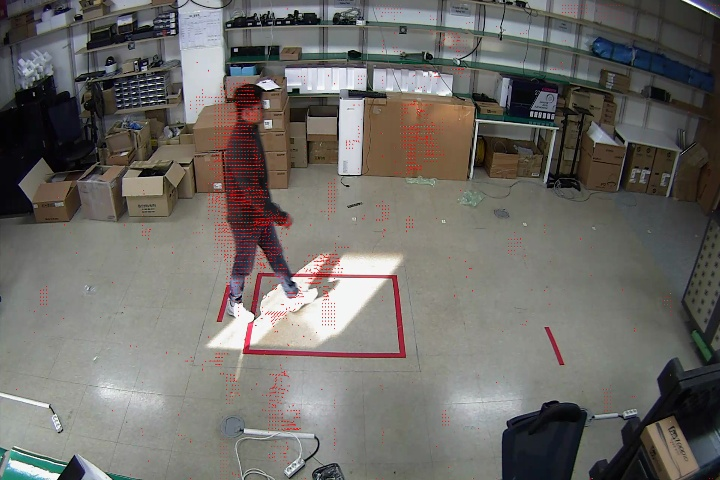
\includegraphics[width=0.25\linewidth]{Figures/1328_mv.jpg}
}
\subfloat[]
{
    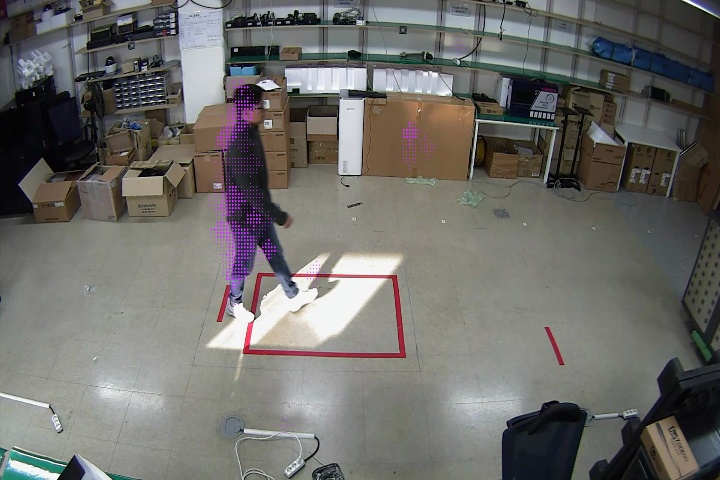
\includegraphics[width=0.25\linewidth]{Figures/1328_occ.jpg}
}
\subfloat[]
{
    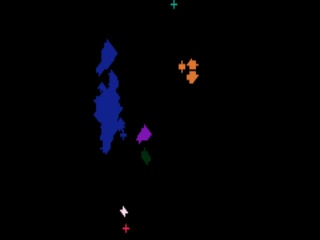
\includegraphics[scale=0.3]{Figures/1328_res.jpg}
}
\subfloat[]
{
    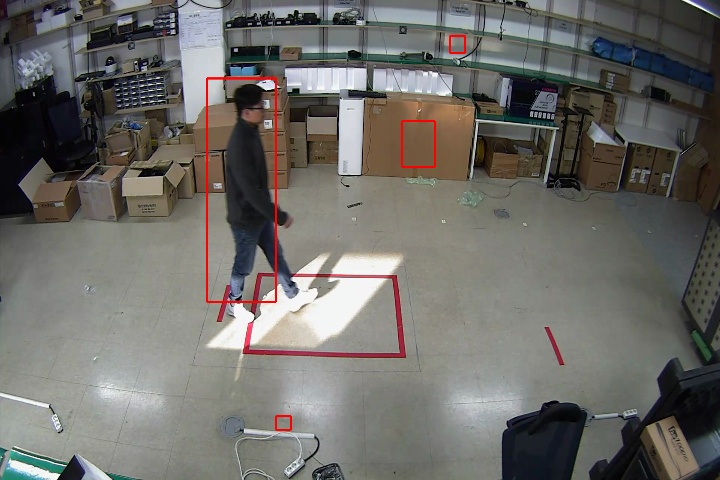
\includegraphics[width=0.25\linewidth]{Figures/1328_obj.jpg}
}\\
\subfloat[]
{
    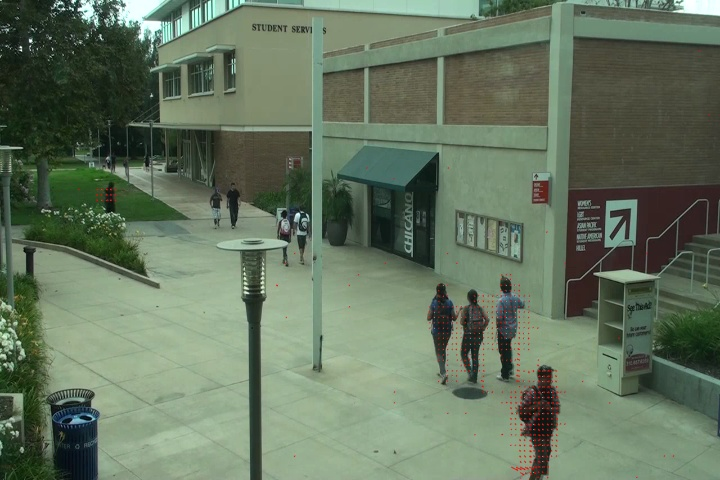
\includegraphics[width=0.25\linewidth]{Figures/38_mv.jpg}
}
\subfloat[]
{
    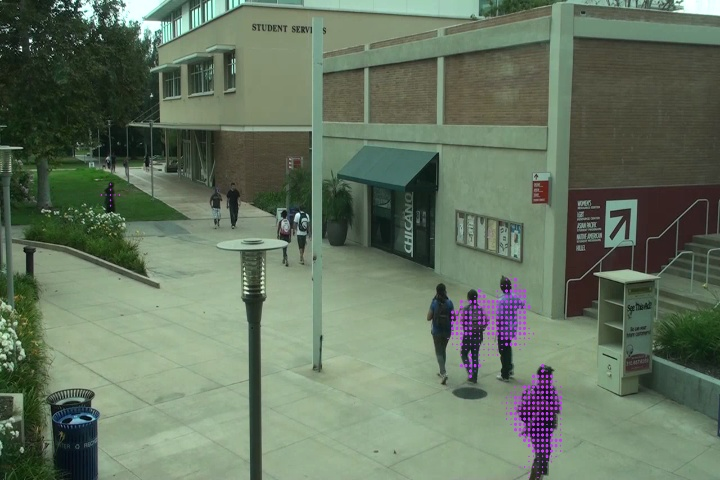
\includegraphics[width=0.25\linewidth]{Figures/38_occ.jpg}
}
\subfloat[]
{
    
\includegraphics[scale=0.3]{Figures/38_res.jpg}
}
\subfloat[]
{
    \includegraphics[width=0.25\linewidth]{Figures/38_obj.jpg}
}
\caption{Moving objects detection by the proposed method with two different video test sequences:(a,e) MV extraction; (b,f) Apply median filter; (c,g) Clustering MVs; (d,f) Blob detection.}
\label{fig:mvanalysis}
\end{figure*}
After clustering, the label list includes all candidate objects with various size, represented by different colors. Typically, the size of candidate object is followed by object size in the video frame. In small object dataset, objects are small when they have mean relative overlap (the overlap area between bounding box area and the image is) from 0.08\% to 0.58\%. Thus, we used a cluster threshold size to filter out the small clustered to the candidate lists as shown in Figure \ref{fig:filter}.\\
\begin{figure*}
\centering
 \includegraphics[width=1.0\linewidth]{Figures/filter.png}
 \caption{Motion size based Filtering}
 \label{fig:filter}
\end{figure*}
After this process, the label list includes the moving objects and certain big MVs noises as shown in Figure \ref{fig:mvanalysis}(c,d). To eliminate these noises, we based the observation on the fact that noise motions because of lighting condition changes usually randomly occur without following a certain flow. Therefore, the tracking motion’s trajectories length is then used to classify the detected motion into the real motion or noise group. If the object tracking trajectory length is larger than a certain threshold, it indicates that the objects move as a flow and the time is sufficiently long to consider it as a real motion. Moreover, I-Frame does not apply motion estimation process, therefore, MV analysis process will be skipped for I-Frames. In order to overcome the discontinuously object detection process, the object tracking algotithm will also be applied to derive the moving object's bounding box in I-frame based on the last states in P-frames. Because the real object moves with a certain flow, the tracking
motion’s trajectories length is then used to classify the candidate
motions into the real motion or noise group, the IoU-based object tracking is applied to track motion because it is light-weight and widely tracking algorithm that calculates the overlap area between two bounding objects. Note that this tracking was implemented and evaluated in some previous studies  \cite{sheu2019stam}, \cite{li2020hksiamfc}. 
\subsection{The IoU based Moving Objects Tracking}
\label{subsec:1}
To apply the IoU-based object tracking, the detected clusters are normalized with a rectangle bounding box according to the cluster's size as shown in Figure \ref{fig:mvanalysis}(d,h). The correlated regions are connected into blobs. Each blob is represented by its top-left and bottom-right corners, i.e.,  ($x_{1}, y_{1}, x_{2}, y_{2}$) may include one or many moving objects. Because the moving object's bounding box size and shape can be different comparatively frame by frame depending on MV’s intensity. Therefore, to track the moving object, an object matching algorithm based on the overlapped area of bounding boxes is applied. We assume that the existence of the real motion is continuous frame by frame. For each bounding box $B_{1}$ in the previous frame, we identify a bounding box $B_{2}$ at the current frame with the highest IoU rate. Note that IoU is attained by:\\
\begin{equation}
\label{eqn:2}
IoU(B_{1}\bigcap B_{2}) = \frac{\left \| B_{1}\bigcap B_{2} \right \|}{\left \| B_{1}\bigcup B_{2}  \right \|} =  \frac{\left \| B_{1}\bigcap B_{2} \right \|}{\left \| \left | B_{1} \right |  +  \left | B_{2} \right |  - B_{1}\bigcap B_{2} \right \|}
\end{equation} 
\begin{figure*}
\centering
 \includegraphics[width=0.4\linewidth]{Figures/iou.png}
 \caption{Object matching method}
 \label{fig:iou}
\end{figure*}
 As its definition in the Equation \ref{eqn:2}, IoU is invariant to the scale, indicating that the similarity between two arbitrary shapes A and B is independent from the scale of their space. The IoU computation’s pseudo-code is given in Algorithm \ref{alg:iou_alg}. If two bounding boxes do not overlap, the IoU value will be 0 and if the IoU score is greater than a detection score threshold ($\alpha$), two bounding boxes are considered in same account (Figure \ref{fig:iou}). The detection score threshold is determined through experiments and depend on the object velocity as well as the distance between objects and camera. Therefore, the method is run with multiple times with different detection score thresholds to tune the best value for each application scenarios. 
\begin{algorithm}
 \caption{ IoU for two bounding boxes.}
 \label{alg:iou_alg}
\SetAlgoLined
\noindent\rule{16cm}{0.4pt}\\
\KwData{ Corners of the two bounding boxes.}
- First bounding box: $A1(x_{1}, y_{1}), B1(x_{2}, y_{1}), C1(x_{2}, y_{2}), D1(x_{1}, y_{2})$\\
- Second bounding box: $A2(x'_{1}, y'_{1}), B2(x'_{2}, y'_{1}), C2(x'_{2}, y'_{2}), D2(x'_{1}, y'_{2})$\\
  where $x_{1} \leq x_{2}, y_{2} \leq y_{1} and  x'_{1} \leq x'_{2}, y'_{2} \leq y'_{1}$.\\
\textbf{Caculation}: IoU value\\
- The area of first bounding box : $Area_{1} = (x_{2} - x_{1})\times (y_{1} - x_{2})$\\
- The area of second bounding box : $Area_{2} = (x'_{2} - x'_{1})\times (y'_{1} - x'_{2})$\\
- The area of overlap: $Area_{overlap} = (max(x_{2}, x'_{2}) - min(x_{1}, x'_{1})) \times (max(y_{2}, y'_{2}) - min(y_{1}, y'_{1})) $\\
- $IoU =\frac{Area_{overlap}}{Area_{1} +  Area_{2} - Area_{overlap}}$\\
\noindent\rule{16cm}{0.4pt}
\
\end{algorithm}
\section{ Performance Evaluated Model}
Computing Resources of VA server is affected by many explicit factors. For example:  whether VA function is running, the complexity of VA function, video resolution, which kind of deep learning model used for VA function, how many cameras is serving. However, the primary factor and biggest effect is number of serving cameras and whether VA function is running. Because if  the VA server is in idle status, then other factors will be implicit. Let assume that we have a video test with N consecutive frames with K frames had the real motion (K<= N).  For each frame, VA server cost S and T unit  of average computing resource  for processing and skip frame case respectively.
For conventional method  of video analytics server, where T = S because all frames are processed , the computing resource average is:\\
\begin{equation}
\label{eqn:3}
Comp_{c}=S
\end{equation}
With our proposed method, the computing resource average during N frames  is calculated as the following equation:\\
\begin{equation}
\label{eqn:4}
Comp_{p}=\frac{(K*S+(N-K)*T)}{N}
\end{equation}
The performance ratio of two method is: \\
\begin{equation}
\label{eqn:5}
\frac{Comp_{p}}{Comp_{c}}=\frac{(K*S+(N-K)*T)}{N*S}=\frac{K}{N} + (1 - \frac{K}{N})*\frac{T}{S}
\end{equation}
if an object motion always appear in the video (K $\approx$ N), then: \\
\begin{equation}
\label{eqn:6}
 \frac{Comp_{p}}{Comp_{c}}\approx 1.
\end{equation}
In case of GPU computing resource, when VA server skip a frame then T = 0 and:\\
\begin{equation}
\label{eqn:7}
\frac{Comp_{p}}{Comp_{c}} = \frac{K}{N}
\end{equation}
 If computing resource is CPU utilization and  network throughput ,  T become very small. For example, T is used only for listening new data or connection with networking resource, then: \\
\begin{equation}
\label{eqn:8}
 \frac{Comp_{p}}{Comp_{c}} \approx \frac{K}{N}
\end{equation}
%!TEX root = ../thesis.tex
%*******************************************************************************
%****************************** Fourth Chapter **********************************
%*******************************************************************************
%Here you make the strongest statement concerning observations. Highlight the information you want readers to remember. Explain how the results correlate with the problems you have indicated in the introduction. Describe all new things that are significant in finding a solution.

%The recommendations part is for giving advice and indicating other actions that will help to solve particular problems. Sound your own opinion about the direction of future research. Most of the time you have to write it. Just like a research proposal.

%Acknowledgments part is a paragraph where you mention everyone who helped you with composition. Place all cited and used information resources into one list or form an annotated bibliography if needed.
\chapter{Implementation And Performance Evaluation}


In this section, the implementation and performance evaluation of the edge-to-clound system with proposed method is presented. Furthermore, the information of video datasets and the scenario setup are provided. In this implementation, VA server executes the application of intrusion detection. Although the evaluated platform integrates specific application, it is a general design and can be extended for other application with few modifications. The workflow of the evaluated platform is represented in Figure \ref{fig:sysdesign}. It has two main components:
\begin{itemize}
\item Edge node implementation: The streaming data from camera sources are parsed and the proposed method is applied to detect moving objects in the current frame. If the encoded frame includes the motion, it will be forwarded to a cloud node using its own real-time streaming protocol (RTSP) server. To avoid decoding inaccuracies at the cloud node, all frames from starting time to ending time of the motion are continuously delivered in a connection session. Each session will start with an intra-coded frame.
\item Cloud node implementation: Receiving the forwarded encoded frame with the motion from the edge node over the network and then decoding and placing the output images into the intrusion detection module, which uses YOLO to detect humans.
\end{itemize} 
\begin{figure*}
\centering
 \includegraphics[width=1.1\linewidth]{Figures/SysDesign.png}
 \caption{Overview of System Design}
 \label{fig:sysdesign}
\end{figure*}
\subsection{Scenario Setup}
\begin{figure*}
 \centering
 \subfloat[]
{
  \includegraphics[width=0.5\linewidth]{Figures/TESTBED.jpg}
}
 \subfloat[]
{
  \includegraphics[scale=0.1]{Figures/pi.jpg}
}
  \caption{Testbed: (a) Scenario Setup, (b) The implemendted edge device.}
  \label{fig:testbed}
\end{figure*}
\begin{table}[]
\centering
\caption{Hardware Specifications.}
\label{tab:hw}
\begin{tabular}{|c|c|c|}
\hline
\textbf{Specifications} & \textbf{Edge Device}   & \textbf{Video Analytics Server}                        \\ \hline
Device Name             & Raspberry Pi 4 & NVIDIA Jetson Xavier                                     \\ \hline
Operating System        & Ubuntu 18.04, 64 bits  & Ubuntu 18.04, 64 bits                                  \\ \hline
GPU                     & Not Supported          & NVIDIA Maxwell architecture with  NVIDIA CUDA cores \\ \hline
CPU                     & Quad-core ARM Cortext-A72          & Quad-core ARM Cortext-A57 MPCore processor             \\ \hline
RAM                     & 4 GB                   & 8 GB                                                   \\ \hline
\end{tabular}
\end{table}
\begin{table}[]
\centering
\caption{Video Test Squence.}
\label{tab:videotest}
\begin{tabular}{|c|c|}
\hline
\multicolumn{2}{|c|}{\textbf{Tested Video Information}} \\ \hline
Resolution                        & 1920x1080           \\ \hline
Length                            & 6 minutes           \\ \hline
Codec                             & H264                \\ \hline
Group Of Picture (GOP)            & 30                  \\ \hline
Frame Rate                        & 25                  \\ \hline
\end{tabular}
\end{table}
\begin{table}[]
\centering
\caption{Testbed: Tested Video Grouth-truth motion time.}
\label{tab:motiontime}
\begin{tabular}{|c|c|}
\hline
\textbf{Time}       & \textbf{Duration (Seconds)} \\ \hline
00:00:50 $~$ 00:01:10 & 20                          \\ \hline
00:01:25 $~$ 00:01:45 & 20                          \\ \hline
00:02:12 $~$ 00:01:10 & 5                           \\ \hline
00:02:39 $~$ 00:02:45 & 6                           \\ \hline
00:03:50 $~$ 00:04:48 & 58                          \\ \hline
00:05:00 $~$ 00:05:35 & 35                          \\ \hline
00:05:40 $~$ 00:06:00 & 20                          \\ \hline
Total               & 164                         \\ \hline
\end{tabular}
\end{table}
\begin{figure*}
\centering
 \includegraphics[scale=0.4]{Figures/ground-truth.png}
 \caption{The ground-truth motion time of our video test sequence.}
 \label{fig:ground}
\end{figure*}
\begin{itemize}
\item Testbed: We built a testbed comprising a single edge device node and a single video analytics server that runs as a cloud node, as shown in Figure \ref{fig:testbed}. The edge device node involves the moving objects detection and runs on a low-computation device named \textit{Raspberry Pi 4} and video analytics server is executed on \textit{Nvidia- Jetson Xavier} because of a GPU that is supported to run YOLO. The hardware specifications of edge node and video analytics server are then listed in Table \ref{tab:hw}. Note that the two devices are directly connected to a router using a wired cable.
\item Video Test Sequence: experiments have been conducted on the two video datasets. The VIRAT video dataset \cite{VIRAT} was collected in natural scenes showing people performing normal actions for video surveillance domains. The second dataset is previously recorded from the our surveillance camera and uploaded \cite{testvideo}. The details of our video test sequence and the ground-truth motion time are shown in Figure \ref{fig:ground} and listed in Tables \ref{tab:motiontime},\ref{tab:videotest}. 
\end{itemize}
We evaluate the performance of the moving object detection method and the proposed edge-to-cloud system separately.

\section{The Light-weight Runtime Moving Object Detection in Video Compressed Domain}
To evaluate the quality of the proposed method for the moving object detection, we calculated the IoU score mettric of the detected object's bounding box with those of the ground-truth bounding box. Because the accuracy of the peoposed method is depend on the MV's density, we run the proposed method multiple times with different scenario application such as: different camera distances, different moving object speeds. We observe that except the I-Frame which does not apply motion estimation, the moving objects including sometimes big MV noises always be detected in other frames. Example of the moving object detection results  are shown in Figure \ref{fig:objectdetect}. 
\begin{figure*}
\centering
\subfloat[]
{
    \includegraphics[scale=0.26]{Figures/1501_res.jpg}
}
\subfloat[]
{
    \includegraphics[width=0.25\linewidth]{Figures/1500_track.jpg}
}
\subfloat[]
{
    \includegraphics[scale=0.26]{Figures/1537_res.jpg}
}
\subfloat[]
{
    \includegraphics[width=0.25\linewidth]{Figures/1536_track.jpg}
}\\
\subfloat[]
{
    \includegraphics[scale=0.26]{Figures/3940_res.jpg}
}
\subfloat[]
{
    \includegraphics[width=0.25\linewidth]{Figures/3939_track.jpg}
}
\subfloat[]
{
    \includegraphics[scale=0.26]{Figures/3949_res.jpg}
}
\subfloat[]
{
    \includegraphics[width=0.25\linewidth]{Figures/3949_track.jpg}
}\\
\subfloat[]
{
    \includegraphics[scale=0.26]{Figures/370_res.jpg}
}
\subfloat[]
{
    \includegraphics[width=0.25\linewidth]{Figures/370_track.jpg}
}
\subfloat[]
{
    \includegraphics[scale=0.26]{Figures/435_res.jpg}
}
\subfloat[]
{
    \includegraphics[width=0.25\linewidth]{Figures/435_track.jpg}
}
\caption{Moving objects detection by the proposed method in different scenarios: (a, b, c, d) human walking; (e, f, g, h) human running; (i, j, k, l) test with a far distance of camera.}
\label{fig:objectdetect}
\end{figure*}

\begin{table}[]
\centering
\caption{Average IoU of the moving object detection in compressed-domain in different scenarios.}
\label{tab:videotest}
\begin{tabular}{|c|c|c|c|}
\hline
\multirow{2}{*}{\textit{\begin{tabular}[c]{@{}c@{}}Video Test\\  Sequence\end{tabular}}} & \multicolumn{2}{c|}{\textit{Scenario}} & \multirow{2}{*}{\textit{IoU Average}} \\ \cline{2-3}
                                                                                         & Camera Position     & Moving Speed     &                                       \\ \hline
Our recorded test video                                                                                        & Near                & Normal           & 0.75                                  \\ \hline
Our recorded test video                                                                                        & Near                & Fast             & 0.26                                  \\ \hline
Video Test from VIRAT                                                                                        & Far                 & Normal           & 0.6                                   \\ \hline
\end{tabular}
\end{table}

\begin{table}[]
\centering
\caption{Average per-frame running times for preprocessing and tracking procedures. Values are expressed in miliseconds (ms) and frame per second(FPS).}
\label{tab:timemessasure}
\begin{tabular}{|c|c|c|c|}
\hline
\textit{Frame Size} & \textit{ST-MRF{[}16{]}} & \textit{Graph Cuts{[}15{]}} & \textit{Proposed Method} \\ \hline
1280x720            & 64 ms (16 FPS)         & 62 ms (17 FPS)              & \textbf{39 ms (26 FPS)}  \\ \hline
1920x1080           & N/A                    & N/A                        & \textbf{69 ms (14 FPS)}  \\ \hline
\end{tabular}
\end{table}
The green bounding boxes shown in the Figure are ground-truth bounding boxes, while the red bounding boxes are detected objects using the proposed method.The average IoU scores are shown in detail for each scenario in Table \ref{tab:videotest}. The results show that when a camera is placed at a close distance and the human does not move fast (i.e, human walking), the proposed method detected well and achieved good average IoU score of 0.75. However, when speed of human is fast in case of running or the camera is in far distance, the MV's density is decreased, the detector return lower average IoU scores. For object tracking evaluation, the scenarios are run with multiple times with different detection score threshold $\alpha$ of 0.25, 0.4 and 0.5 with the results are shown in Figure  \ref{fig:objecttracking}. 
\begin{figure*}
\centering
\subfloat[]
{
    \includegraphics[width=0.3\linewidth]{Figures/1502_025.jpg}
}
\subfloat[]
{
    \includegraphics[width=0.3\linewidth]{Figures/3923_025.jpg}
}
\subfloat[]
{
    \includegraphics[width=0.3\linewidth]{Figures/478_025.jpg}
}\\
\subfloat[]
{
    \includegraphics[width=0.3\linewidth]{Figures/1502_04.jpg}
}
\subfloat[]
{
    \includegraphics[width=0.3\linewidth]{Figures/3923_04.jpg}
}
\subfloat[]
{
    \includegraphics[width=0.3\linewidth]{Figures/478_04.jpg}
}\\
\subfloat[]
{
    \includegraphics[width=0.3\linewidth]{Figures/1502_04.jpg}
}
\subfloat[]
{
    \includegraphics[width=0.3\linewidth]{Figures/3923_05.jpg}
}
\subfloat[]
{
    \includegraphics[width=0.3\linewidth]{Figures/478_05.jpg}
}
\caption{Moving objects tracking by the proposed method with different $\alpha$ thresholds: $\alpha$ = 0.25 in (a, b, c), $\alpha$ = 0.4 in (d, e, f) and $\alpha$ = 0.5 in (d, e, f).}
\label{fig:objecttracking}
\end{figure*}
In this experiment, each $\alpha$ threshold was applied for three same scenarios of human walking in Figure \ref{fig:objecttracking} (a, d, g), human running in Figure \ref{fig:objecttracking} (b, e, h) and the far camera distance in Figure \ref{fig:objecttracking} (c, f, i).  We see that with each test scenario, with lower $\alpha$ threshold value,the tracking object capability is better with longer the object trajactories. However, it will increase the number of false alarm detection if the noise MVs apprear frequently in some specified areas.\\ To optimize the running time speed as well as the performance, the edge node and cloud node all are implemented in C++ using the multithread architecture. We observe that the proposed method does not indicate additional computational difficulty and achieve the approved evaluated results in terms of processing time when compared with previous studies \cite{bombardelli2018efficient} \cite{khatoonabadi2012video}. The average comsuming time  is messasured with different video resolutions and shown in Table \ref{tab:timemessasure}. Compare to other studies, the average processing time for high definition resolution video is approximately 39ms/frame, which outperforms most of the state of art method. This indicates that the proposed algorithm almost handles the data in real-time. 

\section{Performance Evaluation Results}
 In this experiment, the proposed edge-to-clound platform will be implemented and evaluated. Our recored video test sequence is selected because of including different the moving object speeds. Base on the last experiment result shown in Table \ref{tab:videotest}, we choose  $\alpha$ is 0.25 to cover both walking and running case and compared computing resources with the conventional method (no frame filter). The entire demonstration was recorded and uploaded \cite{source}. The evaluated performances of the demonstration are presented in detail as follows.
 
 \subsection{Computing Resources Consumption}
\begin{figure*}
\centering
	\includegraphics[scale=0.35]{Figures/gpu_compare.png}
\caption{GPU Monitoring with the conventional method and the proposed method.}
\label{fig:gpu}
\end{figure*}
\begin{figure*}
\centering
\subfloat[]
{
    \includegraphics[scale=0.7]{Figures/cpu.png}
}
\caption{CPU Monitoring with both the conventional method and the proposed method.}
\label{fig:cpu}
\end{figure*}
\begin{figure*}
\centering
\subfloat[]
{
    \includegraphics[scale=0.7]{Figures/network.png}
}
\caption{Network download throughput monitoring with both the conventional method and the proposed method.}
\label{fig:network}
\end{figure*}
\begin{table}[]
\centering
\caption{Average computing resources of both the conventional method and the proposed method.}
\label{tab:computingresource}
\begin{tabular}{|c|c|c|c|}
\hline
\textbf{Computing Resources}                                         & \textbf{Conventional Method} & \textbf{Proposed Method} & \textbf{Performance Ratio} \\ \hline
GPU Utilization (\%)                                                  & 65.61                        & 33.73                    & 0.51                       \\ \hline
CPU Utilization (\%)                                                  & 50.24                        & 25.9                     & 0.51                       \\ \hline
\begin{tabular}[c]{@{}c@{}}Download Throughput\\ (Kbps)\end{tabular} & 4028                         & 1808.2                   & 0.45                       \\ \hline
\end{tabular}
\end{table}
During demonstration of  intrusion detection application, the clouds node’s computing resources, including CPU, GPU utilization, and network download throughput, was monitored and recorded and shown in Figure \ref{fig:sysdesign}. For comparison, the performance results are compared to that of the conventional method, which did not use edge node as shown in Figure \ref{fig:overall}. The results indicate that both methods achieve the same accuracy in terms of alert notification when humans entered the restricted area. The demonstration's record of both these methods are uploaded to \cite{convential}, \cite{proposed}. In terms of consumption of computational resources, GPU, CPU utilizations, and download throughput of both methods are measured and presented in Figure \ref{fig:gpu}, \ref{fig:cpu} and \ref{fig:network} respectively. The figures clearly show the advantage of using the proposed method. While the conventional method of processing all video frames captured from camera leads to consumption of computational resources, our method only processes when there is motion, and therefore computational resources are dynamically allocated and economical. Another observation is that our proposed method is extremely effective for detecting motion of the scene compared to the ground-truth motion time in Table \ref{tab:motiontime}. In detail,  the time for consuming and releasing computing resources of VA server was matched with the time for appearance and disappearance of motion in ground-truth table. Since the conventional method processes all video frames, we assume that the its computing resource average is S. According to formulation \ref{eqn:5}, the performance ratio of both methods in this video will be as follows:\\
\begin{equation}
\label{eqn:10}
\frac{Comp_{p}}{Comp_{c}}=\frac{(K*S+(N-K)*T)}{N*S}=\frac{K}{N} + (1 - \frac{K}{N})*\frac{T}{S}=\frac{140}{360} + (1 - \frac{140}{360})*\frac{T}{S} = 0.4 + 0.6*\frac{T}{S}
\end{equation}
Compared with the performance ratio, which is calculated in real scenario test in Table \ref{tab:computingresource}, our performance theory model and real measurement are matching and reasonable.
%\include{Chapter5/chapter5}
%\include{Chapter6/chapter6}
%\include{Chapter7/chapter7}



% ********************************** Back Matter *******************************
% Backmatter should be commented out, if you are using appendices after References
%\backmatter

% ********************************** Bibliography ******************************
\begin{spacing}{0.9}

% To use the conventional natbib style referencing
% Bibliography style previews: http://nodonn.tipido.net/bibstyle.php
% Reference styles: http://sites.stat.psu.edu/~surajit/present/bib.htm

\bibliographystyle{apalike}
%\bibliographystyle{unsrt} % Use for unsorted references  
%\bibliographystyle{plainnat} % use this to have URLs listed in References
\cleardoublepage
\bibliography{References/references} % Path to your References.bib file


% If you would like to use BibLaTeX for your references, pass `custombib' as
% an option in the document class. The location of 'reference.bib' should be
% specified in the preamble.tex file in the custombib section.
% Comment out the lines related to natbib above and uncomment the following line.

%\printbibliography[heading=bibintoc, title={References}]


\end{spacing}

% ********************************** Appendices ********************************

%\begin{appendices} % Using appendices environment for more functunality

%%!TEX root = ../thesis.tex
% ******************************* Thesis Appendix A ****************************
\chapter{How to install \LaTeX} 

\section*{Windows OS}

\subsection*{TeXLive package - full version}
\begin{enumerate}
\item	Download the TeXLive ISO (2.2GB) from\\
\href{https://www.tug.org/texlive/}{https://www.tug.org/texlive/}
\item	Download WinCDEmu (if you don't have a virtual drive) from \\
\href{http://wincdemu.sysprogs.org/download/}
{http://wincdemu.sysprogs.org/download/}
\item	To install Windows CD Emulator follow the instructions at\\
\href{http://wincdemu.sysprogs.org/tutorials/install/}
{http://wincdemu.sysprogs.org/tutorials/install/}
\item	Right click the iso and mount it using the WinCDEmu as shown in \\
\href{http://wincdemu.sysprogs.org/tutorials/mount/}{
http://wincdemu.sysprogs.org/tutorials/mount/}
\item	Open your virtual drive and run setup.pl
\end{enumerate}

or

\subsection*{Basic MikTeX - \TeX~ distribution}
\begin{enumerate}
\item	Download Basic-MiK\TeX (32bit or 64bit) from\\
\href{http://miktex.org/download}{http://miktex.org/download}
\item	Run the installer 
\item	To add a new package go to Start >> All Programs >> MikTex >> Maintenance (Admin) and choose Package Manager
\item	Select or search for packages to install
\end{enumerate}

\subsection*{TexStudio - \TeX~ editor}
\begin{enumerate}
\item	Download TexStudio from\\
\href{http://texstudio.sourceforge.net/\#downloads}
{http://texstudio.sourceforge.net/\#downloads} 
\item	Run the installer
\end{enumerate}

\section*{Mac OS X}
\subsection*{MacTeX - \TeX~ distribution}
\begin{enumerate}
\item	Download the file from\\
\href{https://www.tug.org/mactex/}{https://www.tug.org/mactex/}
\item	Extract and double click to run the installer. It does the entire configuration, sit back and relax.
\end{enumerate}

\subsection*{TexStudio - \TeX~ editor}
\begin{enumerate}
\item	Download TexStudio from\\
\href{http://texstudio.sourceforge.net/\#downloads}
{http://texstudio.sourceforge.net/\#downloads} 
\item	Extract and Start
\end{enumerate}


\section*{Unix/Linux}
\subsection*{TeXLive - \TeX~ distribution}
\subsubsection*{Getting the distribution:}
\begin{enumerate}
\item	TexLive can be downloaded from\\
\href{http://www.tug.org/texlive/acquire-netinstall.html}
{http://www.tug.org/texlive/acquire-netinstall.html}.
\item	TexLive is provided by most operating system you can use (rpm,apt-get or yum) to get TexLive distributions
\end{enumerate}

\subsubsection*{Installation}
\begin{enumerate}
\item	Mount the ISO file in the mnt directory
\begin{verbatim}
mount -t iso9660 -o ro,loop,noauto /your/texlive####.iso /mnt
\end{verbatim}

\item	Install wget on your OS (use rpm, apt-get or yum install)
\item	Run the installer script install-tl.
\begin{verbatim}
	cd /your/download/directory
	./install-tl
\end{verbatim}
\item	Enter command `i' for installation

\item	Post-Installation configuration:\\
\href{http://www.tug.org/texlive/doc/texlive-en/texlive-en.html\#x1-320003.4.1}
{http://www.tug.org/texlive/doc/texlive-en/texlive-en.html\#x1-320003.4.1} 
\item	Set the path for the directory of TexLive binaries in your .bashrc file
\end{enumerate}

\subsubsection*{For 32bit OS}
For Bourne-compatible shells such as bash, and using Intel x86 GNU/Linux and a default directory setup as an example, the file to edit might be \begin{verbatim}
edit $~/.bashrc file and add following lines
PATH=/usr/local/texlive/2011/bin/i386-linux:$PATH; 
export PATH 
MANPATH=/usr/local/texlive/2011/texmf/doc/man:$MANPATH;
export MANPATH 
INFOPATH=/usr/local/texlive/2011/texmf/doc/info:$INFOPATH;
export INFOPATH
\end{verbatim}
\subsubsection*{For 64bit OS}
\begin{verbatim}
edit $~/.bashrc file and add following lines
PATH=/usr/local/texlive/2011/bin/x86_64-linux:$PATH;
export PATH 
MANPATH=/usr/local/texlive/2011/texmf/doc/man:$MANPATH;
export MANPATH 
INFOPATH=/usr/local/texlive/2011/texmf/doc/info:$INFOPATH;
export INFOPATH

\end{verbatim}



%\subsection{Installing directly using Linux packages} 
\subsubsection*{Fedora/RedHat/CentOS:}
\begin{verbatim} 
sudo yum install texlive 
sudo yum install psutils 
\end{verbatim}


\subsubsection*{SUSE:}
\begin{verbatim}
sudo zypper install texlive
\end{verbatim}


\subsubsection*{Debian/Ubuntu:}
\begin{verbatim} 
sudo apt-get install texlive texlive-latex-extra 
sudo apt-get install psutils
\end{verbatim}

%%!TEX root = ../thesis.tex
% ******************************* Thesis Appendix B ********************************

\chapter{Installing the CUED class file}

\LaTeX.cls files can be accessed system-wide when they are placed in the
<texmf>/tex/latex directory, where <texmf> is the root directory of the user’s \TeX installation. On systems that have a local texmf tree (<texmflocal>), which
may be named ``texmf-local'' or ``localtexmf'', it may be advisable to install packages in <texmflocal>, rather than <texmf> as the contents of the former, unlike that of the latter, are preserved after the \LaTeX system is reinstalled and/or upgraded.

It is recommended that the user create a subdirectory <texmf>/tex/latex/CUED for all CUED related \LaTeX class and package files. On some \LaTeX systems, the directory look-up tables will need to be refreshed after making additions or deletions to the system files. For \TeX Live systems this is accomplished via executing ``texhash'' as root. MIK\TeX users can run ``initexmf -u'' to accomplish the same thing.

Users not willing or able to install the files system-wide can install them in their personal directories, but will then have to provide the path (full or relative) in addition to the filename when referring to them in \LaTeX.



%\end{appendices}

% *************************************** Index ********************************
\printthesisindex % If index is present

\end{document}
